\chapter{Vorgehen}
\label{ch_vorgehen} 

Das Ziel ist die Entwicklung eines Prototypen aus dem bestehenden Modell der Projektarbeit von \cite{PA_bicycle}. Die Vorgehensschritte sind in der untenstehenden Auflistung abgebildet. Sie bilden die Struktur dieses Kapitels. Die Definition der konkreten Schritte geschah in Absprache mit Prof. Dr. M. Meli und dem Resarch-Assitenten Herr Dario Dünar vom Instiute of Embedded Systems (InES). Auf der CD finden sich die Sitzungsprotokolle über den aktuellen Entwicklungsstand, die offenen Fragen und die Entscheidungen.

\subsubsection*{Liste der Arbeitsschritte}
\label{liste} 

\begin{enumerate}
  \item Inbetriebnahme Machbarkeitsstudie  
  \item Hardware entwickeln  
  \item Inbetriebnahme Prototyp      
  \item Energy und Power Management
  \item Entwickeln einer BLE-Applikation       
 \end{enumerate}  

Die sprachliche Unterscheidung von Energy- und Power-Management entspricht der Unterscheidung zweier ``Management-Teile'' im Prototypen: Das Endprodukt regelt an zwei Stellen auf unterschiedliche Art die zur Verfügung stehende Energie. Der Begriff ``Energy Management'' wird in dieser Arbeit für das Sammeln und Weiterleiten von Energie über eine Hardwareimplementation gebraucht. Der Begriff ``Power Management'' wird für die Softwareimplementation gebraucht. Diese regelt, dass die zur Verfügung gestellte Energie nicht sofort verbraucht wird. Die sprachliche Trennung ist künstlich, denn in der Umsetzung spielen Hard- und Softwareregelung Hand in Hand. Die sprachliche Unterscheidung dient der Lesbarkeit und bezeichnet keinen physikalischen Unterschied.
 
 
 % 1---------------------------------------------------------------------------
 %------------------------------------------------------------------------------
  
 
\section{Inbetriebnahme Machbarkeitsstudie}\label{v_inbetriebnahme} 

      
Ziel der Inbetriebnahme des Aufbaus der vorangehenden Arbeit von \cite{PA_bicycle} ist es, zu definieren, welche Funktionalitäten verbessert werden sollen. Zur Orientierung werden im ersten Unterkapitel \ref{fb} die Funktionsblöcke und deren Aufgaben festgehalten. Danach wird das Verhalten des Vorgängermodells in Unterkapitel \ref{verhalten} ausgemessen. Aus der Analyse entsteht die in Unterkapitel \ref{optimierung} aufgelistete erste Optimierungsliste. Als letztes folgt eine Vertiefung in das auffällige Verhalten des Eingangssignals in Unterkapitel \ref{auffaellig}.
      
\subsection{Funktionsblöcke}\label{fb} 

Der Bicycle Computer besteht aus vier Funktionsblöcken, die in der Abbildung \ref{funktionsdiagramm_bild} dargestellt sind. Der erste Funktionsblock ist der Harvester (siehe 1) in der Abbildung \ref{funktionsdiagramm_bild}). Die Aufgabe des Harvesters besteht darin, Energie zu Ernten und dem nächsten Funktionsblock (Nummer 2) in der Abbildung  \ref{funktionsdiagramm_bild} zur Verfügung zu stellen. Der zweite Funktionsblock wird als Energy Management-Teil in der Arbeit bezeichnet. Die Aufgabe des zweiten Blocks ist es, Energie zu Sammeln und kontrolliert an die Verbrauchsstelle freizuschalten. Detaillierte Informationen finden sich in den Theoretischen Grundlagen im Unterkapitel \ref{t_energy_management}. Der dritte Funktionsblock ist der Ort, an dem die Energie verbraucht wird. In dieser Arbeit dient die Energie dem Betreiben von Sensoren und dem Versenden derer Daten. Dies wird auf dem TI-SensorTag (siehe Anhang \ref{anhang_sensortag}) umgesetzt. Der Grund dafür wird in der Einleitung des Kapitels \label{t_power_management} dargelegt. Der letzte Funktionsblock bezeichnet das Ziel, das Erhalten von Sensordaten in einer Applikation.  


\begin{figure}[ht]
       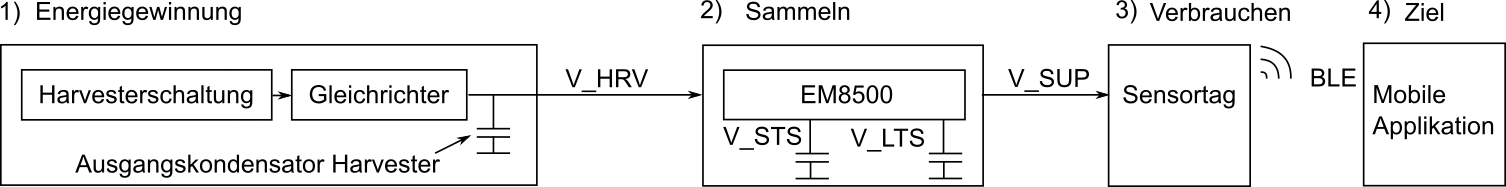
\includegraphics[width=1\textwidth]{3Vorgehen/imag/Blockdiagramm.png}
       \caption{Funktionsblöcke Bicycle Computer}
       \label{funktionsdiagramm_bild}

    \begin{tabbing}
        Bezeichnung \quad\= Beschreibung\\[0.8ex]
        V\_HRV \> Ausgangsspannung Harvesterquelle, Eingangsspannung Energy Management\\
        V\_STS\> Spannung am STS--Kondensator (Primärspeicher)\\
        V\_LTS\> Spannung am LTS--Kondensator (Sekundärspeicher)\\
        V\_SUP\> Ausgangsspannung Energy Managment, Eingangsspannung Sensortag\\
        BLE \> Senden der Daten per Bluetooth Low Energy (siehe \ref{t_ble}) \\
    \end{tabbing} 
\end{figure}

Den Funktionsblöcken sind Spannungsbezeichnungen sowie Kondensatoren beigefügt. Dies, weil bei der Beschreibung des Verhaltens des Vorgängermodells, diese Spannungslevel für die Funktionsbeurteilung wichtig werden.

  

\subsection{Verhalten des Vorgängermodells}\label{verhalten} 

Die Inbetriebnahme bestätigte das in der Dokumentation von \cite{PA_bicycle} beschriebene Verhalten. Die Abbildung \ref{spannungMachbarkeit} zeigt den zeitlichen Verlauf der Energiestände zwischen den Funktionsblöcken (siehe Abbildung \ref{funktionsdiagramm_bild}) und an den Speicherelementen. Die Legende zur Abbildung  \ref{spannungMachbarkeit} erklärt die Signale.

\begin{figure}[ht]
    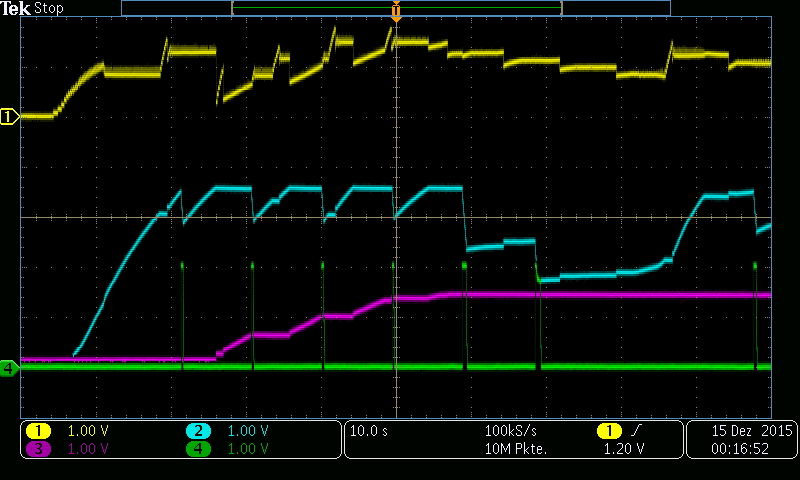
\includegraphics[width=1.0\textwidth]{3Vorgehen/imag/messungPA.png}
    \caption{Spannungswerte Modell der Machbarkeitsstudie}\label{spannungMachbarkeit} 
\begin{tabbing}
    Channel\quad\= Farbe\quad\= Beschreibung\\[0.8ex]
    CH1\> gelb\> Spannungsverlauf V\_HRV\\
    CH2\> blau\> Spannungsverlauf am STS--Kondensator\\
    CH3\> violet\> Spannungsverlauf am LTS--Kondensator\\
    CH4\> grün\> Ausgangsspannung nach Energy Management\\
     \>  \>      Eingangsspannung Sensorttag
\end{tabbing}    
\end{figure}

Im Folgenden werden die einzelnen Spannungsverläufe chronologisch entsprechend der Kanalnummer analysiert. Kanal 1 spiegelt die Spannung am Harvesterausgang wieder (V\_HRV). Gemäss Theorie \ref{eingangsspannung} bzw. gemäss Datenblatt des EM8500 ist der EM8500-Chip für ein DC-Signal ausgelegt. Er geht von einem regelmässigen Eingangssignal aus und regelt die Spannung auf den MPP. Diese Regelung sollte wie in Abbildung \ref{RegelungSpannung} aussehen. Das reale Signal entspricht nicht diesem Verhalten. Die Regelung ist abrupt und überspringt mehrere Spannungslevel. Der Ursache für die schlechte Regelung soll nachgegangen werden.

Kanal 2, blau, gibt den Spannungsverlauf am Hauptspeicher, dem Primärspeicher, der im Datenblatt von EM8500 STS heisst, wieder. Das Energy Management des Vorgängermodells setzt den Schwellwert für den Primärspeicher (STS) mit 3.6 V hoch an. Details zu den Schwellwerten sind im Kapitel Theoretische Grundlagen \ref{t_energy_management} zu finden. Der hohe Wert erklärt sich durch das Ziel, genug Energie für ein konstantes Paketversenden zu haben. Dies gelingt für fünf BLE-Pakete. Danach reicht die Energie nicht mehr aus. V\_SUP, grünes Signal, wird nicht mehr gespiesen. Nach 30 s ohne Pakete senden ist wieder genug Energie für weitere 5 Datenpakete gespeichert.

In der Auswertung fiel uns auf, dass dieser Signalverlauf nur bei einer Geschwindigkeit von 45 km/h möglich ist. Die Speicherkapazität von 470 $\mu$F und ein Schwellwert der Spannung von 3.6 V ist mit normaler Geschwindigkeit (10 km/h) nach 30 min nicht zu erreichen. Fährt man rund 45 km/h so erhält man die in der Abbildung \ref{spannungMachbarkeit} gezeigte Ladezeit von rund 25 s. Eine exakte Geschwindigkeitsmessung ist zu Beginn der Arbeit nicht möglich. Das Rad wird von Hand gedreht und mit einem Metronom wird die Umdrehungsgeschwindigkeit vorgegeben. Bei einem Radumfang von 2.04 m und einer Zeitdifferenz von 160 ms zwischen den Reed-Impulsen, ergibt sich die Geschwindigkeit von ca. 45 km/h. Da diese Messmethode über längere Zeit nicht sehr genau ist, bestand eine der Aufgaben nach der Inbetriebnahme im Organisieren eines Messaufbaus. Dieser professionellere Messaufbau wird im Anhang \ref{messaufbau} beschrieben.

Kanal 3, das rosa Signal, zeigt die Spannung am Long-Time-Speicher. Die Inbetriebnahme zeigt, dass sich der LTS lädt. Es erstaunt jedoch, dass seine geerntete Energie nicht verwendet wird. Der Spannungswert von LTS geht nie herunter.
Die Vermutung ist, dass der eingestellte Schwellwert für den Bezug von Energie von LTS (siehe Abbildung \ref{energiespeisung_lts}) nicht stimmt.

Kanal 4, das grüne Signal zeigt die Speisung des TI-SensorTags. Im Modell der Projektarbeit steuert der Mikrokontroller des Sensortags den Verbrauch. Alle 10 s wacht das System auf, bezieht Energie vom EM8500-Ausgang für das Senden eines Paketes und geht dann wieder schlafen. Das Aufwachintervall ist fix.


\subsection{Optimierungsliste}\label{optimierung} 

Aus den Messungen der Inbetriebnahme konkretisierten sich die generellen Aufgaben, die in der ersten Liste der Arbeitsschritte zu Beginn des Vorgehens  beschrieben wurden. Nachfolgende vier Punkte sollen durch den Prototypen verbessert werden: 

\begin{minipage}{1\textwidth}
\begin{itemize}
     \item Der Verlauf des Harvester-Eingangs wechselt abrupt. Der Eingang soll besser geregelt werden. 
     \item Für das Laden des Primärspeichers von 470 $\mu$F in 25 s benötigt es eine Geschwindigkeit von mehr als 60 km/h.  Die Harvesterschaltung soll so weiterentwickelt werden, dass bei 10 km/h genug Energie zum Senden von BLE-Paketen besteht.    
     \item Das zweite Speicherelement, der LTS, entlädt sich nicht. Dadurch kann seine Energie nicht verwendet werden. Die Schwellwerte am EM8500 und ev. die Kondensatorenwerte sollen so angepasst werden, dass sich der zweite Kondensator entlädt
     \item Die Energie wird statisch nach einem fixen Zeitintervall von 10 s genutzt. Das Zeitintervall soll der Geschwindigkeit angepasst werden. Bei höherer Geschwindigkeit soll das Intervall kürzer werden.
\end{itemize} 
\end{minipage}

Im Resultatsteil Kapitel \ref{ch_resultat} werden die Fortschritte in diesen vier Punkten ausgewiesen.

\subsection{Vertiefung Harvesterausgang}\label{auffaellig} 

Herr Ives Théoduloz hatte uns im Rahmen eines Besuchs auf die Problematik, einer zu grossen Kapazität am Eingang des EM-Chips, hingewiesen. Laut seiner Aussage sollte der Kondensator am Eingang des EM-Chips, bzw. dem Ausgang des Harvesters am besten kleiner sein als 4.7 $\mu$F. Bisher wurde im Aufbau der Machbarkeitsstudie ein Kondensator mit 470 $\mu$F verwendet. Herr Ives Théoduloz meinte, dass dieser Kondensator viel zu gross sei und dass die Regelung am Eingang des EM-Chips möglicherweise nicht richtig funktionieren würde. Daher wurde dieses Problem näher untersucht und in mehreren Schritten optimiert.

Im ersten Schritt wurde der Kondensator verkleinert, bis die Rippelspannung noch annehmbar war. Die Rippelspannung bei dem bestehenden Kondensator von 470 $\mu$F beträgt ca. 10 mVpp. Die Rippelspannung bei einer Kapazität von 47 $\mu$F beträgt bereits ca. 40 mVpp, jedoch ist die Rippelspannung noch in einem Bereich der annehmbar scheint. Bei einer Kapazität von 10 $\mu$F liegt die Rippelspannung bei ca. 500 mVpp. Die Abbildung \ref{47uF_mit_Limiter_AC} veranschaulicht die Rippelspannung von einem Kondensator mit 47 $\mu$F, die Abbildung \ref{10uF_mit_Limiter_DC} zeigt die Rippelspannung über einem Kondensator von 10 $\mu$F.

\begin{figure}[ht]
 \begin{minipage}[t]{0.5\textwidth}
    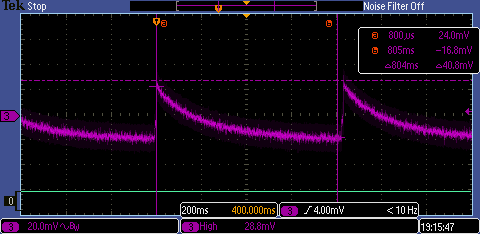
\includegraphics[width=0.90\textwidth]{3Vorgehen/imag/47uF_mit_Limiter_AC.PNG}
    \caption{Rippelspannung über dem 47 $\mu$F Kondensator}
	\label{47uF_mit_Limiter_AC} 
 \end{minipage}
 \begin{minipage}[t]{0.5\textwidth}
    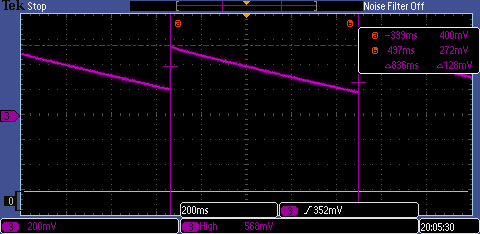
\includegraphics[width=0.90\textwidth]{3Vorgehen/imag/10uF_mit_Limiter_DC.PNG}
    \caption{Rippelspannung über dem 10 $\mu$F Kondensator}
	\label{10uF_mit_Limiter_DC} 
 \end{minipage}
\end{figure}

Jedoch muss auch ein Blick auf die Spannung am Harvesterausgang geworfen werden, wenn dieser Ausgang mit dem EM-Chip belastet wird. Es kann beobachtet werden, dass der Eingang des EM-Chips ein fluktuierendes Spannungslevel (siehe Abbildung \ref{VCC_47uF_15kmh_Periode}) erhält. 

\begin{figure}[ht]
   \begin{minipage}[t]{0.5\textwidth}
     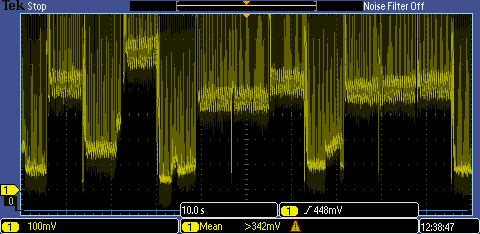
\includegraphics[width=0.90\textwidth]{3Vorgehen/imag/VCC_47uF_15kmh_Periode.PNG}
     \caption{Spannung am EM8500-Eingang über einem 47 $\mu$F Kondensator}
	 \label{VCC_47uF_15kmh_Periode}
  \end{minipage}
  \begin{minipage}[t]{0.5\textwidth}
    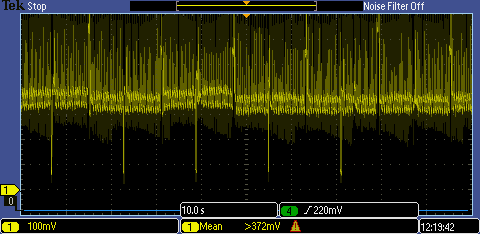
\includegraphics[width=0.90\textwidth]{3Vorgehen/imag/VCC_100uF_15kmh_Periode.PNG}
    \caption{Spannung am EM8500-Eingang über einem 100 $\mu$F Kondensator}
	\label{VCC_100uF_15kmh_Periode}
  \end{minipage} 
\end{figure}

Problematisch ist, dass die Spannung am Eingang des EM8500-Chip wiederholt unter die 0.3 V Grenze fällt, bei einer Spannung von 0.3 V kann keine Energie gespeichert werden. Die Regelung am Eingang des EM-Chips kann mit der anliegenden Rippelspannung nicht richtig arbeiten. Die Rippelspannung muss verringert werden, bzw. die Kapazität am Ausgang des Harvesters muss erhöht werden. 

Das Problem ist, dass durch den Rippel die periodische Open-Loop-Spannungsmessung keine korrekten Messwerte erhält. Sobald die Last vom Harvesterausgang abgehängt wird, steigt die Spannung über dem Kondensator, jedoch wird die Open-Loop-Spannung bei einer grossen Kapazität nicht erreicht, da die Zeit, bis der Kondensator komplett geladen ist, sehr gross ist. Jedoch bedeutet eine niedrige Kapazität, dass die Rippelspannung relativ hoch ist und je nach Zeitpunkt der Open-Loop-Messung eine andere Spannung am Kondensator ergibt. Die Spannung am Kondensator steigt bei jeder Messung auf ein anderes Spannungslevel.

Es musste ein Kompromiss gefunden werden, so dass die Spannung am Eingang des EM-Chips auf ein konstantes Level geregelt werden kann. Die Kapazität des Kondensators sollte nicht zu klein sein, damit der Rippel nicht zu gross wird. Andererseits darf der Kondensator nicht zu gross sein, da ansonsten die Open-Loop-Messung keine richtigen Werte liefert. Den Kompromiss stellt der 100 $\mu$F Kondensator dar, bei diesem ist die Spannung am Eingang relativ konstant und es kann damit gearbeitet werden (siehe Abbildung \ref{VCC_100uF_15kmh_Periode}).

Aus den Beobachtungen ergaben sich folgende Aufgaben für die Entwicklung des Prototypen:

\begin{enumerate}
    \item Die Harvesterschaltung funktioniert nicht optimal. Die Auswirkung des zu hohen Kondensator vor Harvestereingang soll getestet werden
    \item Die Schaltung soll für eine Geschwindigkeit von 10 km/h ausgelegt werden
    \item Die Konfigurationen beim EM8500 sollen überarbeitet werden, sodass LTS genutzt wird
    \item Das Senden der Pakte soll der Geschwindigkeit angepasst werden
\end{enumerate}

Punkte 1 und 2 haben Auswirkung auf das Layout, Punkte 3 und 4 auf die Entwicklung des Energymanagements und der Firmware für das TI-SensorTag.


%------------------------------------------------------------------------------
% 2---------------------------------------------------------------------------
%------------------------------------------------------------------------------



\section{Hardware entwickeln}

Aus der Inbetriebnahme der Machbarkeitsstudie wurden einige Punkte ersichtlich, welche mit einer neuen Leiterplatte, bzw. einer neuen Hardware verbessert werden können. Im speziellen muss die Harvesterschaltung genauer angeschaut werden und es soll versucht werden, die nachfolgenden Punkte aus der Inbetriebnahme der Machbarkeitsstudie umzusetzen. 

\textit{Die Schaltung soll für eine Geschwindigkeit von 10 km/h ausgelegt werden.}

Ausserdem soll die neue Leiterplatte den fliegenden Aufbau der Harvesterschaltung und den EM-Chip beherbergen. Es wird in diesem Schritt darauf verzichtet, das TI-SensorTag ebenfalls in die neue Leiterplatte zu integrieren. Die Hardware kann gut in mehreren Schritten überarbeitet werden.

\subsection{Das Schema}

Bevor ein Leiterplattenlayout entwickelt werden kann, muss das Schema gezeichnet werden. Es wurden verschiedenste Vorgaben von den Dozenten vorgegeben, welche im besten Fall alle eingehalten werden. 

\begin{enumerate}
    \item Die Grösse der Leiterplatte soll die Grösse des TI-SensorTags nicht überschreiten.
    \item Alle Netze sollen mit Testpunkten ausgestattet werden.
    \item Alle Anschlüsse des TI-SensorTags sollen auf der Leiterplatte zugänglich sein.
    \item Alle Testpunkte des TI-SensorTags sollen im Rastermass 2.5 mm angeordnet werden.
	\item Strommesspunkte sollen an der Speisung des TI-SensorTags, des Longterm Storage und des Shortterm Storage angebracht werden. (optional)
\end{enumerate}

Diese Vorgaben sollen die Leiterplatte für eventuelle Laborübungen der Schule verwendbar machen. Das Schema besteht in den Grundzügen aus vier Teilen:

\begin{enumerate}
    \item Harvesterschaltung
    \item EM-Chip inklusive zugehöriger Peripherie
    \item Energiespeicher
    \item Umlauferfassung
\end{enumerate}

\subsubsection{Harvesterschaltung}

Die Harvesterschaltung wurde in der Machbarkeitsstudie als fliegender Aufbau realisiert, was zu einigen Problemen führen kann, da viele lange Kabel verwendet wurden und somit die Signallaufwege lang sind. Bisher hat dies keine Probleme verursacht, doch es geht wichtige Energie in den Kabeln verloren. Ebenfalls wurde in der Inbetriebnahme bemerkt, dass die gewonnene Leistung sehr gering ist, weswegen die Schaltung in einem zweiten Schritt optimiert werden muss.

\begin{figure}[ht]
    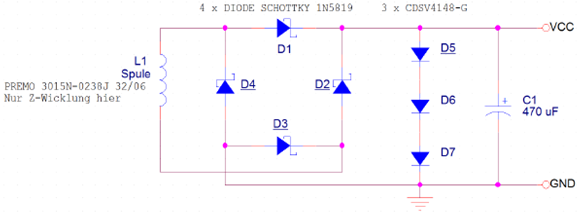
\includegraphics[width=0.5\textwidth]{3Vorgehen/imag/Schema_Harvester_PA.png}
    \caption{Harvesterschaltung der PA15(\cite{PA_bicycle})}
    \label{schema_harvester_pa15} 
\end{figure}

Die Harvesterschaltung der Abbildung \ref{schema_harvester_pa15} wurde im Rahmen der Machbarkeitsstudie erarbeitet. Die Schaltung besteht aus wenigen Teilen, die Spannungbegrenzung wurde mit drei Dioden in Durchlassrichtung realisiert, hier gibt es wahrscheinlich bessere Möglichkeiten die Spannung zu begrenzen, ohne Leistung zu verschwenden.

\subsubsection{EM8500-Chip}

Das EM-Evaluationsboard soll ebenfalls auf der neuen Leiterplatte Platz finden, das Schema inklusive aller Kondensatoren ist im Datenblatt zu finden. Jedoch wurden die Jumper nicht übernommen und nur einige Stecker wurden übernommen, bzw. mit eigenen Signalen ergänzt (siehe Abbildung \ref{schema_em-chip_inkl_peripherie}).


\begin{figure}[ht]
    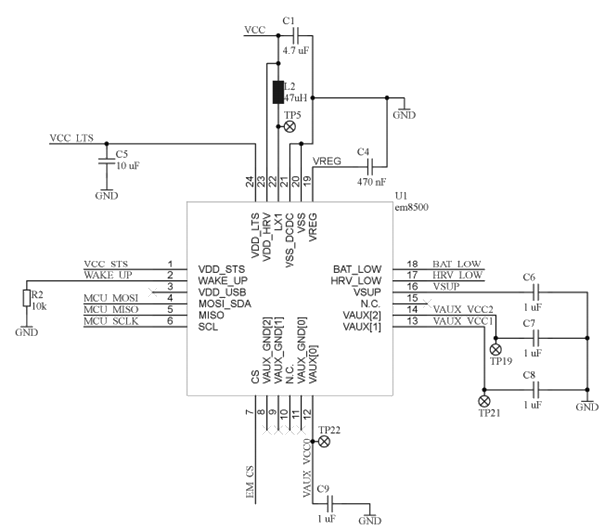
\includegraphics[width=1.0\textwidth]{3Vorgehen/imag/Schema_EM-Chip_inkl_Peripherie.png}
    \caption{Schema des EM-Chips mit der benötigten Peripherie}\label{schema_em-chip_inkl_peripherie} 
\end{figure}

\clearpage
\subsubsection{Energiespeicher}

Die Energiespeicher waren zum Zeitpunkt der Entwicklung der Hardware noch nicht definiert. Als Platzhalter wurden zwei Elektrolytkondensatoren (ElKo) mit den Werten aus der Machbarkeitsstudie eingefügt (siehe Abbildung \ref{schema_energiespeicher}). 

\begin{figure}[ht]
    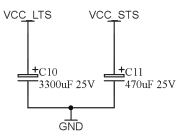
\includegraphics[width=0.3\textwidth]{3Vorgehen/imag/Schema_Energiespeicher.png}
    \caption{Schema der Energiespeicher (ElKos sind nur Platzhalter)}
    \label{schema_energiespeicher} 
\end{figure}


\subsubsection{Umlauferfassung}

Die Umlauferfassung kann nicht mit der verwendeten Spule realisiert werden, da bei der Energiegewinnung mit der Spule, das Signal gleichgerichtet wird. Die nicht benutzten Wicklungen der X- und Y-Wicklung liefern kein verwertbares Signal, was bereits in der Machbarkeitsstudie bewiesen wurde. Aus diesem Grund wird der Magnetdurchlauf mit einem Reed Switch detektiert und an das TI-SensorTag weitergegeben (siehe Abbildung \ref{schema_umlaufdetektion}). Ein Magnetdurchlauf erzeugt einen positiven Puls, solange sich der Magnet in der Reichweite des Reed Switch befindet.

\begin{figure}[ht]
    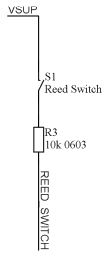
\includegraphics[width=0.1\textwidth]{3Vorgehen/imag/Schema_Umlaufdetektion.png}
    \caption{Schema Umlauferfassung}\label{schema_umlaufdetektion} 
\end{figure}

\subsection{Bauteildefinition und Optimierung}

Nachdem klar war, welche Teile auf der Leiterplatte Platz finden müssen, konnte die Optimierung der Schaltung in Angriff genommen werden. Ziel der Optimierung war es, bei 10 km/h genügend Energie zu gewinnen, damit das TI-SensorTag damit versorgt werden könnte. Dafür musste vor allem die Harvesterschaltung optimiert werden, damit keine Energie verloren geht. 
Es wurden folgende Punkte angeschaut und versucht zu optimieren:

\begin{enumerate}
    \item die Spule
    \item der Gleichrichter
    \item der Limiter
\end{enumerate}

\subsubsection{Die Spule}

Die Spule gewinnt die Energie aus dem an einer Speiche des Fahrrads befestigten Magneten. Eine stärkere Spule könnte mehr Energie aus dem vorbei schnellenden Magneten gewinnen. Entscheidend ist das die Fläche der Spule nicht vergrössert werden darf, bestenfalls sollte eine kleinere Spule gefunden werden, welche mehr Energie gewinnt. Gemäss der Formel 2.4 ist für die gewonnene Energie vor allem die Wicklungszahl entscheidend, jedoch wird bei den Spulen meistens nur die Induktivität angegeben. Die Induktivität hängt quadratisch von der Wicklungszahl und linear von der Fläche (siehe Formel \cite{equ_inductivity}) ab.

\begin{equation}
	L = \mu_0 \times \frac{N^2\times A}{l}
\end{equation}

Es wurde nach einer Spule mit einer höheren Induktivität und der gleichen Fläche gesucht, somit können nur noch zwei Variablen sich verändern. Zum einen kann sich die Wicklungszahl verändern und zum andern kann sich die Länge der Spule verändern. Die Spule von Würth Elektronik mit der Bezeichnung 74458308 hat eine ähnliche Fläche und eine grössere Induktivität, was auf den ersten Blick sehr vielversprechend aussieht.

Die Messung der erzeugten Spannung über der Spule hat ergeben, dass die Spule von Premo mit der Bezeichnung 3015N 0238J 3206, welche bisher verwendet wurde, eine höhere Spannung erzeugt als die neue Spule von Würth. Die Spule von Premo hat bei den Geschwindigkeiten von 10 km/h und 20 km/h eine grössere induzierte Spannung. Die Spule von Würth hat eine höhere Spannung bei den Geschwindigkeiten von 15 km/h und 40 km/h. Jedoch sollte die Schaltung für 10 km/h optimiert werden, somit wird der Spule von Premo der Vortritt gewährt. Nachfolgend wird der Unterschied zwischen den induzierten Spannungen in den Spulen ersichtlich (siehe Abbildungen \ref{messung_optimierung_spule} und \ref{blublu}). Der Unterschied ist nicht gross, jedoch muss hier die Spule von Premo bevorzugt werden, da die induzierte Spannung grösser ist.

\begin{figure}[ht]
 \begin{minipage}[t]{0.5\textwidth}
    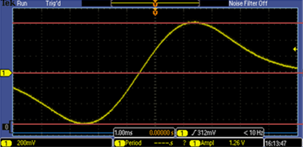
\includegraphics[width=0.9\textwidth]{3Vorgehen/imag/Messung_Optimierung_Spule_links.png}
    \caption{Spule von Premo}               
    \label{messung_optimierung_spule} 
 \end{minipage}
 \begin{minipage}[t]{0.5\textwidth}
    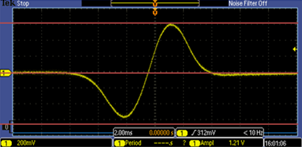
\includegraphics[width=0.9\textwidth]{3Vorgehen/imag/Messung_Optimierung_Spule_rechts.png}
    \caption{Spule von Würth}  
    \label{blublu}             
 \end{minipage}
\end{figure}

\subsubsection{Der Gleichrichter}

Der Gleichrichter aus der Machbarkeitsstudie bestand aus vier Dioden vom Typ 1N5819. Diese Dioden sind nicht für die Low-Power-Anwendung ausgelegt, ausserdem sind die Dioden nicht in einem Gehäuse verbaut. Wichtig ist bei dem Gleichrichter, dass die Leckströme möglichst klein sind und die Schwellenspannung sollte ebenfalls möglichst klein sein, damit wenig Energie verbraucht wird.

Es wurde als erstes eine Low-Power-Diode, mit der Bezeichnung HSMS-286P, getestet. Die Erwartungen waren entsprechend hoch, da diese Dioden für Low-Power-Anwendungen spezialisiert sind. Die Spule von Premo wurde als Quelle verwendet, um zu sehen, wie die Spannung nach dem Gleichrichter aussieht. Die Spannung nach dem Gleichrichter bestehend aus den Dioden vom Typ 1N5819 ist bei allen getesteten Geschwindigkeiten, also 10 km/h, 15 km/h, 20 km/h und 40 km/h, höher als beim Gleichrichter bestehend aus den Dioden vom Typ HSMS-286P. Der Spannungsunterschied liegt im Minimum bei ca. 40 mV. Der grösste Unterschied ist bei der Geschwindigkeit von 15 km/h ersichtlich, was in den Abbildungen \ref{messung_optimierung_gleichrichter_1} und \ref{pling} gezeigt wird.

\begin{figure}[ht]
 \begin{minipage}[t]{0.5\textwidth}
    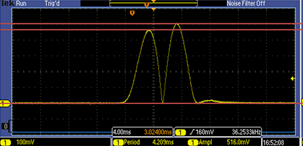
\includegraphics[width=0.9\textwidth]{3Vorgehen/imag/Messung_Optimierung_Gleichrichter_1_links.png}
    \caption{Gleichrichter 1N5819}
    \label{messung_optimierung_gleichrichter_1} 
 \end{minipage}
 \begin{minipage}[t]{0.5\textwidth}
    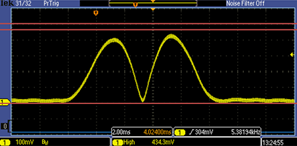
\includegraphics[width=0.9\textwidth]{3Vorgehen/imag/Messung_Optimierung_Gleichrichter_1_rechts.png}
    \caption{Gleichrichter HSMS-286P}
    \label{pling}
 \end{minipage}
\end{figure}

Als nächstes wurde ein Gleichrichter aus den Dioden vom Typ BAT54 getestet. Die Spannung nach dem Gleichrichter bestehend aus 1N5819 Dioden ist bei den Geschwindigkeiten von 15 km/h, 20 km/h und 40 km/h höher als nach dem Gleichrichter bestehend aus BAT54 Dioden. Der Spannungsunterschied liegt bei ca. 100 mVpp. Der Unterschied ist marginal, jedoch muss hier der Gleichrichter aus 1N5819 Dioden bevorzugt werden. Nur bei einer Geschwindigkeit von 10 km/h ist der Gleichrichter bestehend aus BAT54 Dioden besser als der Gleichrichter bestehend aus 1N5919 Dioden. Der Spannungsunterschied liegt hier bei ca. 10 mVpp. Dieser Unterschied ist vernachlässigbar, in Angesicht dessen, dass der Gleichrichter bestehend aus 1N5819 Dioden in allen anderen getesteten Geschwindigkeiten besser ist.

\begin{figure}[ht]
 \begin{minipage}[t]{0.5\textwidth}
    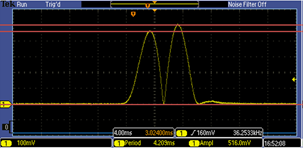
\includegraphics[width=0.9\textwidth]{3Vorgehen/imag/Messung_Optimierung_Gleichrichter_2_links.png}
    \caption{Gleichrichter 1N5819}
    \label{messung_optimierung_gleichrichter_2} 
 \end{minipage}
 \begin{minipage}[t]{0.5\textwidth}
    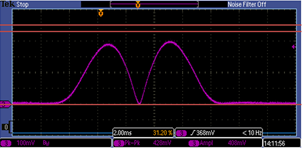
\includegraphics[width=0.9\textwidth]{3Vorgehen/imag/Messung_Optimierung_Gleichrichter_2_rechts.png}
    \caption{Gleichrichter BAT54}
 \end{minipage}
\end{figure}

\subsubsection{Der Limiter}

Die Spannungsbegrenzung, nachfolgend der Limiter genannt, ist ein sehr krititscher Teil der Harvesterschaltung, da die Spannung am EM-Chip Eingang nicht höher als 2 V sein darf, da ansonsten der EM-Chip beschädigt werden kann. Trotzdem soll möglichst wenig Energie verloren gehen, wenn die Spannungsbegrenzungsschaltung ihre Arbeit verrichtet. Bisher wurden drei Dioden in Durchlassrichtung in Serie geschaltet, um die Spannung zu begrenzen.

Herr Erich Ruff hat eine Spannungsbegrenzungsschaltung entwickelt, welche er uns freundlicherweise zur Verfügung stellte. Diese Schaltung wurde mit dem Limiter verglichen, welcher aus drei Dioden bestand.

Die Spannung nach dem Dioden-Limiter ist bei 10 km/h, 15 km/h und 20 km/h höher, jedoch ist die Rippelspannung ebenfalls höher. Nur bei einer Geschwindigkeit von 40 km/h ist die Spannung nach dem Limiter von Herr Erich Ruff, nachfolgend FET-Limiter genannt, besser, sowohl bei Spannungslevel als auch bei der Rippelspannung. Die Abbildung \ref{messung_optimierung_limiter} zeigt, dass der Dioden-Limiter eine höhere Spannung liefert, jedoch ist die Rippelspannung ebenfalls höher.

\begin{figure}[ht]
 \begin{minipage}[t]{0.5\textwidth}
    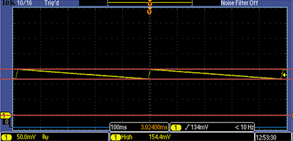
\includegraphics[width=0.9\textwidth]{3Vorgehen/imag/Messung_Optimierung_Limiter_links.png}
    \caption{Dioden-Limiter}
    \label{messung_optimierung_limiter} 
 \end{minipage}
 \begin{minipage}[t]{0.5\textwidth}
    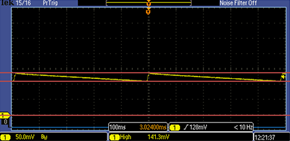
\includegraphics[width=0.9\textwidth]{3Vorgehen/imag/Messung_Optimierung_Limiter_rechts.png}
    \caption{FET-Limiter}
 \end{minipage}
\end{figure}

\subsection{Layout}

Schlussendlich musste aus den optimierten Teilen des Schemas eine Leiterplatte gestaltet werden. Die meisten Footprints waren bereits in den Bibliotheken des InES vorhanden, einige mussten neu gezeichnet werden.

\subsubsection{Positionierung}

Die Positionierung der einzelnen Teile kann sehr wichtig sein, da mit einer guten Positionierung bereits unnötige Leiterbahnverläufe verhindert werden können. Ebenfalls können gut positionierte Bauteile die Spannungspegel stabilisieren. Es wurde darauf geachtet, dass die Bauteile, welche zu einem Block gehören, nahe beieinander zu platzieren, um unnötig lange Signallaufwege zu verhindern.

Die Bauteile der Harvesterschaltung wurden als Block so nahe wie möglich beieinander platziert und wo immer möglich wurden die Speisungsleitungen mit einer Leiterbahnbreite von 20 Mil gezogen, damit der Widerstand der Leiterbahn (\cite{eqn_res_leiter}) möglichst klein gehalten wurde. Der Leiterwiderstand konnte so minimiert werden, was verhindert, dass die Energie in den Leiterbahnen verschwendet wird.

\begin{equation}
	R = \rho \times \frac{l}{A}
\end{equation}

Der Widerstand bei 10 Mil ist somit ca. 1.9 m$\Omega$ pro Meter, 
der Leiterwiderstand bei einer Leiterbahnbreite von 20 Mil ist ca. 1.0 m$\Omega$ pro Meter. Problematisch ist, dass sich der Block der Harvesterschaltung etwas entfernt vom Block des EM-Chips befindet. Das bedeutet, dass die Leiterbahn mit der Speisung des EM-Chips mehrere Zentimeter zurücklegen muss. Sicherlich ist der Unterschied im Widerstand nicht sehr gross, doch die Energie, welche in der Leiterbahn verloren gehen würde, konnte so halbiert werden.

Der wichtigste Aspekt der Platzierung des EM-Chips war, dass die Stützkondensatoren so nah wie möglich am EM-Chip platziert wurden, damit die Spannung am EM-Chip so konstant wie irgend möglich gehalten werden kann.

\begin{minipage}{1\textwidth}
Ein wichtiger Punkt ist die Platzierung des Steckers, welcher unsere Leiterplatte mit dem TI-SensorTag verbindet. Durch eine Falschplatzierung kann es hier passieren, dass die beiden Leiterplatten nicht korrekt übereinander ausgerichtet sind, wenn sie aufeinander gesteckt werden. Das ist eher ein ästhetisches Problem, jedoch kann das auch Probleme beim Einbauen in ein Gehäuse bereiten. Zu dem Stecker gehört auch die Platzierung der Testpunkte, welche direkt mit dem Stecker verbunden sind. Gemäss dem Wunsch der Betreuer wurde hier ein Rastermass von 2.5 mm der Testpunkte eingehalten, so dass eine Steckerleiste eingelötet werden könnte. Problematisch ist jedoch, dass die Testpunkte einen grossen Raum der Leiterplatte einnehmen, wie in Abbildung \ref{layout_testpunkteraster} ersichtlich.
\end{minipage}

\begin{figure}[ht]
    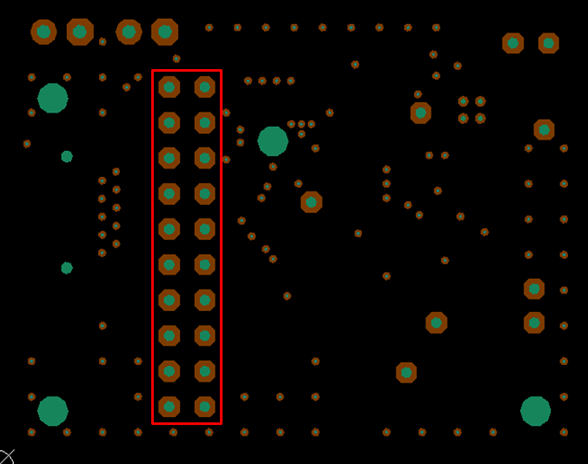
\includegraphics[width=0.8\textwidth]{3Vorgehen/imag/Layout_Testpunkteraster.png}
    \caption{Pads der Leiterplatte, rot eingerahmt die Testpunkte des Steckers}\label{layout_testpunkteraster} 
\end{figure}

\subsubsection{Das erste Layout}

Die erste Version der Leiterplatte war mit vielen Forderungen der Betreuer ausgestattet. Alle Netze wurden mit Testpunkten ausgestattet. Die Testpunkte des Steckers wurden im Rastermass 2.5 mm angeordnet und die Netze der Spannung nach dem Harvester, die Spannung des Short- und Long-Term-Storage wurden mit Strommesspunkten ausgestattet. Es wurden ebenfalls Montagelöcher platziert, jedoch sind diese sehr minimalistisch, da nur eine M2-Schraube durchpasst. Besser wäre es, Montagelöcher für M3-Schrauben zu platzieren, doch der Platz auf der Leiterplatte ist sehr limitiert. Die Leiterplatte ist nur 33 x 42 mm gross, was ein Milimeter breiter ist als das TI-SensorTag. Der Anschluss der Energiespeicher wurde so realisiert, dass die Energiespeicher nicht auf der Leiterplatte Platz finden, da der Platz nicht ausreicht.


\subsubsection{Das Redesign}

Das Layout wurde von Herr Olivier Rion begutachtet. Seine Kritikpunkte werden auf der nächsten Seite aufgelistet.

\newpage
\begin{minipage}{1\textwidth}

Kritikpunkte am Schema:
\begin{enumerate}
    \item VCC sollte in Pfeil sein: Das Symbol für VCC und generell alle Speisungen sollten als Pfeil im Schema dargestellt werden.
    \item Generell für eine erste Version sind viele TP gut.
    \item Auf dem Schema fehlt noch ein Symbol für die GND Pads für Messungen: Auf dem Top-Layer des Layouts wurde eine Fläche von Lötstopplack freigestellt, dies sollte auf dem Schema verzeichnet werden.
	\item Die freien Pins auf X1 sollten mit IO angeschlossen sein: Die nicht verwendeten Pins vom EM8500-Chips sollten mit dem Stecker X1 verbunden werden, jedoch ist das problematisch, da eine direkte Verbindung zum Mikroprozessor Energie verbrauchen kann, solange der Mikroprozessor nicht gestartet ist.
	\item Unten links auf dem Schema fehlt die Versionen, die Beschreibung, usw.
	\item Eine kleine Beschreibung beim Harvester wäre gut, z.B. Prinzip mit T1, Spannungsregulierung usw.: Eine Beschreibung hilft die Schaltung schneller zu verstehen, dass macht eine Übergabe an die nachfolgenden Studenten einfacher.
\end{enumerate}


Kritikpunkte am PCB:
\begin{enumerate}
    \item Die Grenze vom Print sollte mit Mechanical und keepOutLayer gemacht werden.
    \item Loch oben links: Die Leiterbahnen sind zu nah um die Löcher platziert, es sollte ein keepOutLayer um die Löcher platziert werden.
    \item Die Leiterbahnen sollten immer in Gruppen platziert werden.
	\item GND kann Kontakt mit den Schraubenköpfen haben: Es muss sichergestellt werden, dass die Schraube keinen Kontakt mit den Leitungen hat und dass die Flächen nicht unter dem Schraubenkopf platziert werden. 
\end{enumerate}

Wir sind dankbar für konstruktive Kritik, jedoch kann diese Kritik aus zeitlichen Gründen noch nicht umgesetzt werden. Neben den Kritikpunkten von Herr Rion wurden während der Arbeit noch weitere Kritikpunkte ersichtlich.

\begin{enumerate}
    \item Die Testpunkte auf der Leiterplatte müssen neu platziert werden, weil sie Teilweise auf der Unterseite nicht angelötet werden können, da die Spule sie verdeckt. 
    \item Die Abstände zwischen den Testpunkten müssen vergrössert werden, damit eine KO-Sonde gut daran befestigt werden kann ohne einen Kurzschluss zu verursachen.
    \item Der Footprint vom Stecker X1 muss überarbeitet werden, da dieser falsch erfasst wurde.
	\item Die Position des Steckers X1 muss verändert werden, da die Position nicht mit dem Gegenstück des TI-SensorTags übereinstimmt.
	\item Die Netze VCC\_STS, VCC\_LTS und VREG dürfen nicht mit dem Stecker X1 verbunden werden, da die Energie über diese Anschlüsse verloren geht.
\end{enumerate}
\end{minipage}

\newpage
Die Punkte 3 bis 5, welche den Stecker X1 betreffen konnten vor Abschluss noch überarbeitet werden, jedoch wäre die Lieferzeit für die Leiterplatte zu lang, als dass die Leiterplatten vor Abgabe der Arbeit eintreffen würden. Darum wurden alle Messungen mit der ersten Version der Leiterplatte durchgeführt.


% 4----------------------------------------------------------
\section{Inbetriebnahme des Prototypen}

Nach der Entwicklung der neuen Hardware musste diese getestet werden, um die Funktionsweise mit den bisherigen Messungen zu verifizieren. Es werden generell zwei wichtige Messstellen (siehe Abbildung \ref{EnergieMessungStellen}) ersichtlich. Die erste befindet sich nach dem Harvester und vor dem EM8500-Chip, die zweite wichtige Messstelle befindet sich zwischen dem EM8500-Chip und dem TI-SensorTag. Es ist wichtig die Leistungs- oder Energiemessung durchzuführen, da diese Werte essentiell für die Einstellung des EM8500-Chips und die Entwicklung der Firmware für das TI-SensorTags sind. 

\begin{figure}[ht]
  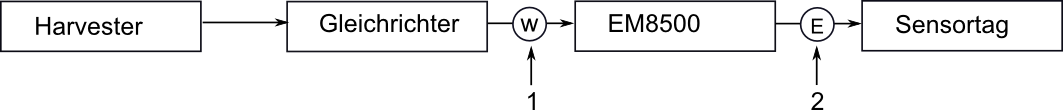
\includegraphics[width=1.0\textwidth]{3Vorgehen/imag/EnergiemessungStellen.png}               
  \caption{Messstellen am Prototypen}
  \label{EnergieMessungStellen} 
\end{figure}

\subsection{Testen der Harvesterschaltung}
\label{glace}

\subsubsection{Leistungsverifizierung}
\label{leistungsverifizierung}

Es wurde eine Leistungskennline der Harvesterschaltung aufgenommen, um die verfügbare Leistung zu verifizieren. Wichtig ist, dass die verfügbare Leistung im gleichen Bereich ist, wie beim fliegenden Aufbau. 

\begin{minipage}{1\textwidth}
\captionof{table}{Leistung des fliegenden Aufbaus}
\label{tab:leistung_fliegenden-aufbaus} 
\begin{tabbing}
    Geschwindigkeit   \quad\= maximale Leistung    \quad\= MPP-Ratio\\[0.8ex]
    10 km/h        \> 12.87 $\mu$W  \> 43.23 \%\\
	20 km/h        \> 43.35 $\mu$W  \> 45.51 \%\\
	40 km/h        \> 250.26 $\mu$W  \> 48.44 \%
\end{tabbing}
\end{minipage}

\begin{minipage}{1\textwidth}
\captionof{table}{Leistung der neuen Leiterplatte}
\label{tab:leistung_neuen_leiterplatte} 
\begin{tabbing}
    Geschwindigkeit   \quad\= maximale Leistung    \quad\= MPP-Ratio\\[0.8ex]
    10 km/h        \> 10.17 $\mu$W  \> 56.99 \%\\
	20 km/h        \> 48.57 $\mu$W  \> 61.82 \%
\end{tabbing}
\end{minipage}

Die maximal zur Verfügung stehende Leistung wurde etwas kleiner, bei dem fliegenden Aufbau betrug die maximale Leistung bei 10 km/h ca. 12 $\mu$W, die maximale Leistung bei der neuen Leiterplatte beträgt ca. 10 $\mu$W. Jedoch ist bei einer Geschwindigkeit von 20 km/h die Leistung der neuen Leiterplatte besser und der MPP wurde ebenfalls verschoben, was ein grosser Vorteil ist, da die Einstellung des MPPT-Ratio auf dem EM8500-Chip konfiguriert werden kann. Bisher konnte das MPPT-Ratio nicht korrekt auf die Hardware eingestellt werden, da die Einstellung nur Werte zwischen 50\thinspace\% und 80\thinspace\% akzeptiert.

\subsubsection{Testen der Spule}\label{starkeSpule}

Es wurde klar, dass die Energie, welche die Harvesterschaltung mit der aktuellen Spule von Premo mit einer Induktivität von 2.38 mH liefert zu klein ist und verbessert werden muss. Ideen wurden gesammelt und Herr Marcel Meli bemerkte, dass noch eine Spule von Premo mit einer Induktivität von 4.77 mH vorhanden wäre, diese sollte getestet werden. Die Spule hatte den exakt gleichen Aufbau wie die Spule, welche bis anhin verwendet wurde, nur die Induktivität war höher. Gemäss der Formel \cite{equ_inductivity} ist die Induktivität von der Wicklungszahl abhängig. Die Wicklungszahl wiederum beeinflusst die induzierte Spannung.

\captionof{table}{Leistung mit unterschiedlichen Spulen}
\begin{tabbing}
    Spule\hspace{2cm}   \quad\= maximale Leistung    \\[0.8ex]
    Premo 2.38 mH        \> 48.57 $\mu$W\\
	Premo 4.77 mH        \> 66.82 $\mu$W\\
	
\end{tabbing}

Die Messung hat ergeben, dass die Energie bei einer Verdoppelung der Induktivität eine Leistungssteigerung von ca. 37\thinspace\% zur Folge hat. Dies lässt sich auch mathematisch nachweisen:

\begin{flalign}
	&L = \mu_0 \times \frac{N^2\times A}{l}\\
	&N = \sqrt{\frac{L\times l}{\mu_0\times A}}\\
	&neue\,Wicklungszahl = \sqrt{2} \times bisherige\,Wicklungszahl
\end{flalign}

Da die Leistung von der induzierten Spannung abhängt und die induzierte Spannung von der Wicklungszahl abhängt, steigt die Leistung in Abhängigkeit zur Wicklungszahl. Ein Zuwachs der Leistung von bis zu 41\thinspace\% war zu erwarten. Es wurde entschieden, dass die stärkere Spule mit einer Induktivität von 4.77 mH verwendet werden soll.

\subsubsection{Testen Magnete in Serie}

Herr Dario Dündar machte uns auf ein Produkt von Reelight aufmerksam. Die Firma Reelight stellt Lichter für das Fahrrad her welche über Energy Harvesting betrieben werden, dafür werden neben der Wirbelstromvariante (siehe Unterkapitel Ausgangslage \ref{ausgang}) ebenfalls Produkte mit speziellen Magneten verwendet. Leider war kein Datenblatt für die Magnete mit der Bezeichnung RE-10200 vorhanden und auch auf Nachfrage wurde kein Datenblatt oder Ähnliches herausgegeben. Jedoch konnte man herausfinden, dass in dem Gehäuse drei Magnete verbaut sind, welche stärker sind als unsere Magnete. Unsere Magnete haben eine N42 Magnetisierung, was bedeutet, dass sie eine Remanenz von 1.29 – 1.32 Tesla haben. Die Magnete, welche im Gehäuse von Reelight verbaut sind, haben eine N45 Magnetisierung, was bedeutet sie haben eine Remanenz von 1.37 – 1.42 Tesla. Der Durchmesser der Magnete beträgt 2.5 mm. Unsere bisher verwendeten Magnete wiesen einen Durchmesser von 20 mm auf.
 

Es wurde eine Leistungskennlinie mit dem Magneten von Reelight aufgenommen. Die maximale zur Verfügung stehende Leistung betrug 135.50 $\mu$W, was einem Zuwachs von über 100\thinspace\% entsprach.\\

\captionof{table}{Leistung mit unterschiedlicher Anzahl an Magneten}
\begin{tabbing}
    Konfiguration\hphantom{4.77 mH, 3 Magnete in Serie (Reelight)}   \quad\= maximale Leistung    \\[0.8ex]
    Spule Premo 4.77 mH, 1 Magnet in Serie        \> 66.82 $\mu$W\\
	Spule Premo 4.77 mH, 3 Magnete in Serie (Reelight)        \> 135.50 $\mu$W\\
\end{tabbing}

Diese Messung brachte uns auf die Idee einen weiteren Versuch zu realisieren. Wir modifizierten den Testaufbau, damit zwei Magnete direkt hintereinander montiert werden konnten. Es sollte untersucht werden, ob die beiden Magnete die Spule besser anregten als nur ein Magnet. Die induzierten Spannungswerte unterschieden sich nicht drastisch, jedoch wurde die Spule länger angeregt. Die Abbildungen \ref{zweiMagneteInSerie} und \ref{manu} zeigen den Unterschied zwischen einer Spule, welche nur von einem Magneten angeregt wurde und einer Spule, welche von zwei direkt aufeinander folgenden Magneten angeregt wurde. Es ist zu sehen, dass die Spannung in der Spule, welche nur mit einem Magneten angeregt wurde, höher ist, jedoch wesentlich kürzer anliegt. Es wurde, trotz dem Potential für mehr Energie mit zwei Magneten, dagegen entschieden zwei Magnete in Serie einzusetzen, da man dieses Prinzip wieder ins Extreme treiben könnte und das ganze Rad mit Magneten ausstatten könnte. Sicherlich würde das jegliches Energieproblem unserer Arbeit lösen, jedoch wäre dies unpraktisch, wegen der verstärkten Bremswirkung und es wäre unästhetisch.

\begin{figure}[ht]
 \begin{minipage}[t]{0.5\textwidth}
  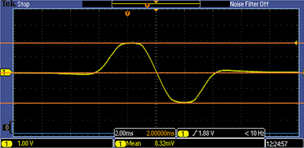
\includegraphics[width=0.9\textwidth]{3Vorgehen/imag/zweiMagneteInSerie_links.png}
  \caption{Anregung der Spule mit einem Magneten}
  \label{zweiMagneteInSerie} 
 \end{minipage}
 \begin{minipage}[t]{0.5\textwidth}
  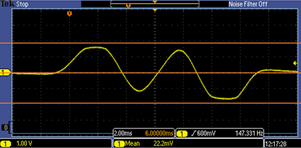
\includegraphics[width=0.9\textwidth]{3Vorgehen/imag/zweiMagneteInSerie_rechts.png}
  \caption{Anregung der Spule mit zwei Magneten in Serie}
  \label{manu}
 \end{minipage}
\end{figure}


\subsection{Ausmessen der Leistung der endgültigen Hardware}

Gemäss dem vorangegangen Unterkapitel \ref{glace} Abschnitt \ref{starkeSpule} wurde ersichtlich, dass die stärkere Spule verwendet werden sollte. Wir haben uns jedoch gegen die Variante mit zwei Magneten in Serie entschieden, trotzdem könnte dies später verwendet werden. Es musste erneut die Leistung, welche die Harvesterschaltung zur Verfügung stellt, aufgenommen werden.\\


\begin{minipage}{\textwidth}
\captionof{table}{Leistung des Prototypen}
\begin{tabbing}
    Geschwindigkeit   	\quad\= maximale Leistung    \\[0.8ex]
    10 km/h		        \> 24.77 $\mu$W\\
	15 km/h		        \> 61.07 $\mu$W\\
	20 km/h		        \> 116.69 $\mu$W\\
	40 km/h		        \> 472.61 $\mu$W\\
\end{tabbing}
\end{minipage}

Die maximal verfügbare Leistung konnte durch die stärkere Spule erneut deutlich verbessert werden. 

\subsection{Ausmessen der Energieabgabe EM8500-Chip}
\label{em_enerige_ausgang}

Es war nun bekannt, wie viel Leistung die Harvesterschaltung zur Verfügung stellte, jedoch musste die Leistungsabgabe nach dem konfigurierten EM8500-Chip noch erfasst werden. Diese Angabe war sehr wichtig, um die Entwicklung der Firmware zu optimieren. Diese Werte gaben einen Rahmen, wie viel Energie das TI-SensorTag verbrauchen durfte.\\

Da es sich beim Ausgang des EM8500-Chips um eine Spannungsquelle handelt, welche bei uns auf 2 V konfiguriert wurde, konnte man die Energie, welche zur Verfügung stand, messen. Der Ausgang des EM8500-Chips wurde für diesen Zweck mit einem 10 k$\Omega$ Widerstand belastet. Anschliessend wurde gemessen, wie lange die Spannung am Ausgang aufrecherhalten werden konnte. Die Abbildung \ref{EnergieEMChip15kmh} zeigt den Spannungsverlauf über der Last. Da der Spannungsverlauf annähernd ein Rechteck war, konnte die Energie anhand der Zeit, welche der Ausgang aktiv war, berechnet werden.

\begin{equation}
	E = \frac{U^2}{R}  \times \Delta t
\end{equation}

\begin{figure}[ht]
  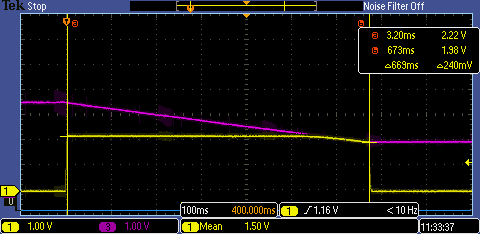
\includegraphics[width=0.80\textwidth]{3Vorgehen/imag/EnergieEMChip15kmh.PNG} 
  \caption{rot: VCC\_STS, gelb: VSUP}
   \label{EnergieEMChip15kmh} 
\end{figure}



\captionof{table}{Leistungsabgabe Ausgang EM8500}
\label{tab:em_out_zsm}
\begin{tabbing}
    Geschwindigkeit   	\quad\= abgegebene Energie    \\[0.8ex]
    10 km/h		        \> 261.2 $\mu$Ws\\
	15 km/h		        \> 267.6 $\mu$Ws\\
	20 km/h		        \> 273.2 $\mu$Ws\\
	40 km/h		        \> 373.2 $\mu$Ws\\
\end{tabbing}

% 5---------------------------------------------------------------------------
\section{Energy Management}

Das Ziel des Energy Managements ist es, dass die zur Verfügung stehende Energie bei 10 km/h genügt, um BLE-Pakete zu versenden. Die sekundäre Aufgabe ist es, dass sich der LTS lädt und entlädt. Ein Laden des LTS ohne dass die Energie im LTS verwertet werden kann ist Energieverschwendung. Die zwei gestellten Aufgaben sollen durch möglichst optimale Speichergrössen und intelligente Schwellwerte erreicht werden.\\

Damit man die Kondensatorenwerte berechnen kann, braucht es Energiedaten. Deshalb stehen als erstes im Unterkapitel \ref{v_messungen_sensortag} die Energie-Messergebnisse, danach folgt im zweiten Unterkapitel \ref{v_e_kalkulation} die Dimensionierung der Kondensatoren und dann das Berechnen der Schwellwerte in Unterkapitel \ref{v_schwellwerte}. Als letzer Punkt werden die Energiezustände innerhalb des Bicycle Computers definiert. Dies, weil die letzte offene Aufgabe der Optimierungsliste (\ref{optimierung}) das Senden nach 10 s dem Energiezustand angepasst werden soll.


% x.1 ------------------------
\subsection{Energiemessungen}
\label{v_messungen_sensortag}


Die Entwicklung ist konstant begleitet durch Energiemessungen. Sei dies durch Leistungsmessungen bei der Hardware (Harvester und EM8500-Chip) oder sei dies als Energiemessung der Software (TI-SensorTag). Für die Energiemessungen wird der Power Analyser von Agilent Electronic N6705B verwendet. Dieses Messgerät misst gleichzeitig Strom, Spannung und Leistung im Zeitverlauf. Annäherungen aus den Messungen mit einem Oszilloskop sind nicht mehr notwendig.\\

In diesem Unterkapitel werden die Resultate den TI-SensorTag-Energiemessungen dargestellt. Mehr Messgrafiken und Erklärungen sind im Messprotokoll (\cite{messung_energie_sensortag}) abgelegt. Den Überblick über die Versionen ist in der untenstehenden Tabelle aufgelistet. 


\subsubsection{Überblick Energiemessungen}\label{erst_EMessungen}

\begin{figure}[ht]
    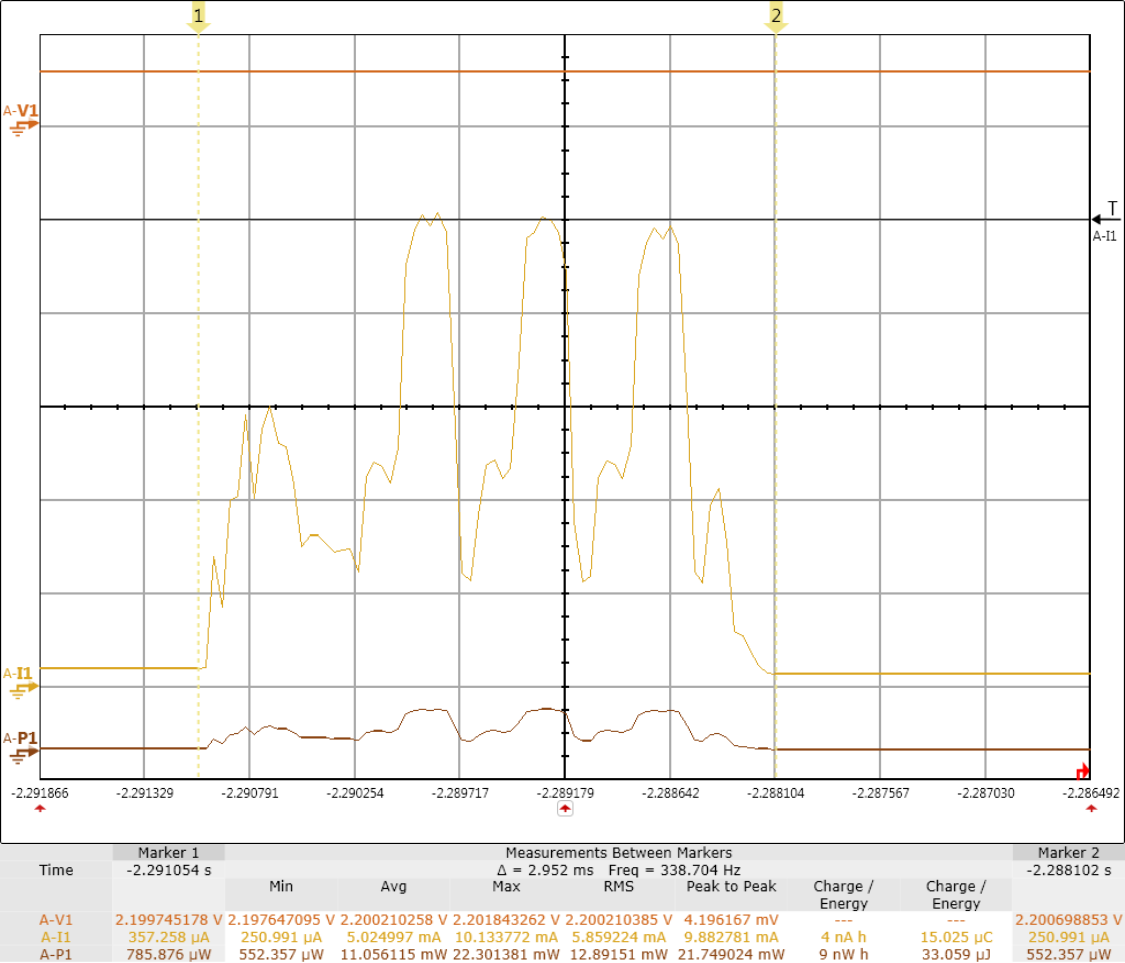
\includegraphics[width=1.0\textwidth]{3Vorgehen/imag/v0Send33uJ.png} 
    \caption{3 BLE Pakte im Advertising Mode}
    \label{BLE_send}
\end{figure}

Um einen ersten Anhaltspunkt über den Energieverbrauch des TI-SensorTags zu erhalten, werden drei BLE-Pakete im Advertsing Mode per Knopfdruck gesendet (siehe Abbildung \ref{BLE_send}). Dies entspricht der Messung zur TI-SensorTag-Version V0. Nach der Weiterentwicklung des Programms zum Auslesen der Sensoren, folgte die Messung der Version V1. In dieser Version wird die GPIO ausgelesen. Die GPIO ist für das Einlesen der Reed Switch-Impulse unumgänglich. Die Version V2, der Versuch mehr Sleep-Time einzubauen, scheitert am Zusammenspiel des Timings der BLE-Radio-Interrupts mit den GPIO-Interrupts. Durch das Neuaufsetzen des Programms entsteht die Version V3. Diese sendet power-optimiert Geschwindigkeitspakete.\\ 

Die untenstehende Tabelle stellt die Energieresultate dar. Unterschieden wird zwischen dem Energieverbrauch für die Initialisierung, kurz Init, und der Energie zum Senden von drei BLE-Paketen. Die Diskussion über Energieoptimierungen und die Deutung der Resultate finden sich in den Sitzungsprotokollen (\cite{sitzungsprotokoll_160226}, \cite{sitzungsprotokoll_160516_ms3}).\\

\begin{minipage}{\textwidth}
\captionof{table}{Messresultate nach TI-SensorTag-Versionen}
\begin{tabbing}
    Version   \quad\= Datum    \quad\= Aufgabe\hphantom{re ohne Schlafmodus} \quad\= Energie Init    \quad\=  Energie Senden \\[0.8ex]
    V0        \> 10.3.16  \> Nur BLE Paket      \> unbekannt            \> 33 $\mu$J \\
    V1        \> 16.3.16  \> mit Geschwindigkeit      \> 87 $\mu$J            \> 32 $\mu$J \\
    V3        \> 22.4.16   \> Schlafmodus optimiert     \> 40 $\mu$J            \> 29 $\mu$J \\
    V4        \> 03.6.16    \> 3 Sensore ohne Schlafmodus   \> 77 $\mu$J            \> 43 $\mu$J \\
    V5        \> ongoing    \> 3 Sensore mit Schlafmodus     \> unbekannt           \> unbekannt\\
\end{tabbing}
\end{minipage}

Bei den ersten drei Messungen werden die Sensoren noch nicht ausgelesen. Es zeigt sich, dass das Auslesen der Sensoren über I2C und das Warten, bis die Sensoren gestartet sind,  mehr Energie verbraucht als erwartet. Der Energieverbrauch für das Auslesens eines Sensors ist ohne Optimierungsmassnahmen so gross, dass kein Senden der Daten möglich ist. Die Speisung der Applikation bricht zusammen (siehe Abbildung \ref{i2c_problem}).

\begin{figure}[ht]
    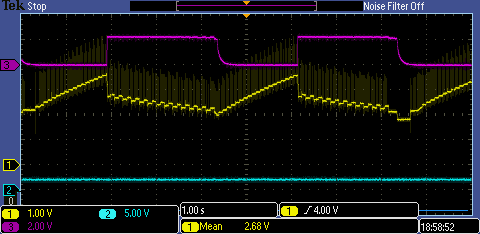
\includegraphics[width=0.5\textwidth]{3Vorgehen/imag/pic4VSUPbrichtEin.PNG} 
    \caption{Energieeinbruch beim Auslesen der Sensoren}
    \label{i2c_problem}
\end{figure}

\begin{minipage}{1\textwidth}
Aus diesen Grund wurde die Poweroptimierung innerhalb des Programms zur zentralen Herausforderung in dieser Arbeit. Details darüber sind im nächsten Unterkapitel (\ref{powerOptimierung} Power Management) zusammengefasst. Bei der Version V4 zeigt sich, dass die Funktion BLE-Send, zu der auch das Einlesen der Sensordaten gehört, einen Zuwachs von 50\thinspace\% an Energiebedarf bewirkt. 
\end{minipage}


\subsubsection{Resultate Energieverbrauch TI-SensorTag Applikation V4}
\label{energie_sensortag} 

Als Überblick über den konkreten Energieverbrauch bei der Version V4 (siehe Messprotokoll \cite{messung_energie_sensortag}) folgt exemplarisch ein Bild zur Initialisierung (Abbildung \ref{energie_init}), eines zum Senden der drei BLE-Pakete (Abbildung \ref{energie_senden}) und dann je eine Abbildung zum Energieverbrauch beim Starten der drei Sensoren. Die Abbildung \ref{energie_ueberblick} zeigt den Überblick eines erstmaligen Sendens. Ganz links ist das einmalige Aufladen der Kondensatoren auf dem TI-SensorTag zu sehen. Dieser Vorgang ist in Abbildung \ref{energie_kondensatoren_sensortag} vergrössert dargestellt. Aus der Abbildung \ref{energie_ueberblick}, die den Überblick des Sendens darstellt, kann man die durchschnittliche Zeit, nach der ein Refresh erfolgt ungefähr herauslesen. Durchschnittlich folgt ca. alle 0.1 s ein Refresh-Peak. Auch dieser Vorgang ist als einzelne Energiemessung aufgenommen und in Abbildung \ref{energie_refresh} dokumentiert. Am Schluss dieses Unterkapitels werden alle Energiewerte in einer Tabelle zusammengefasst.

\begin{figure}[ht]
  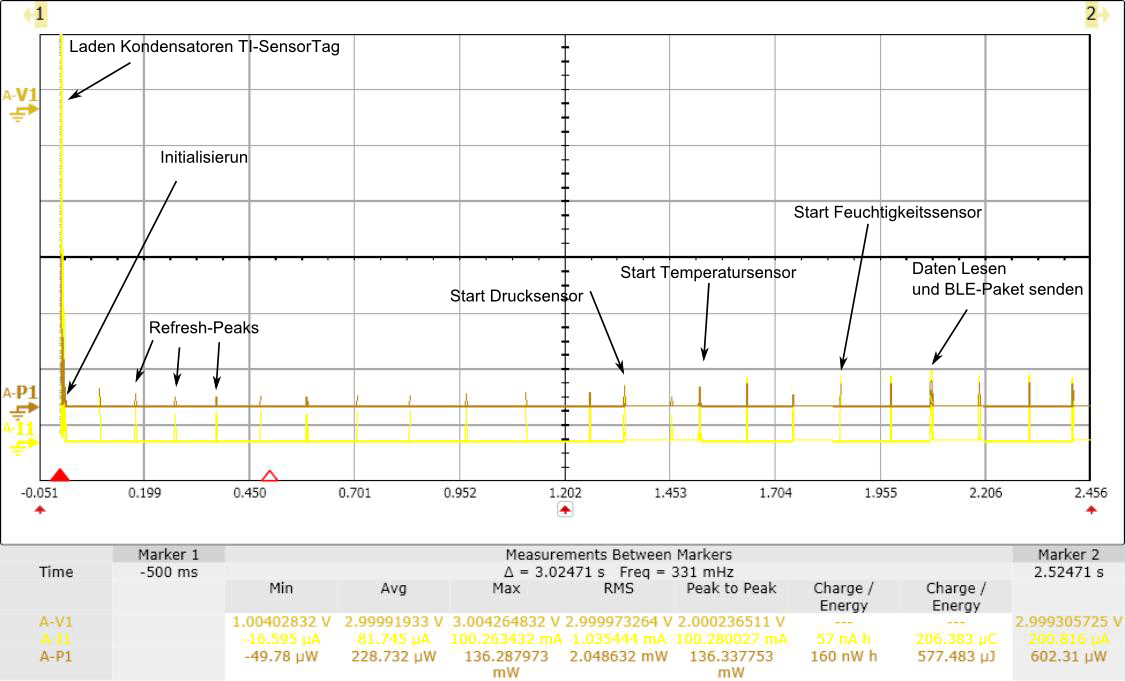
\includegraphics[width=1.0\textwidth]{3Vorgehen/imag/Ueberblick.png}
  \caption{Überblick Energieverbrauch}
  \label{energie_ueberblick}
\end{figure}

\begin{figure}[ht] 
  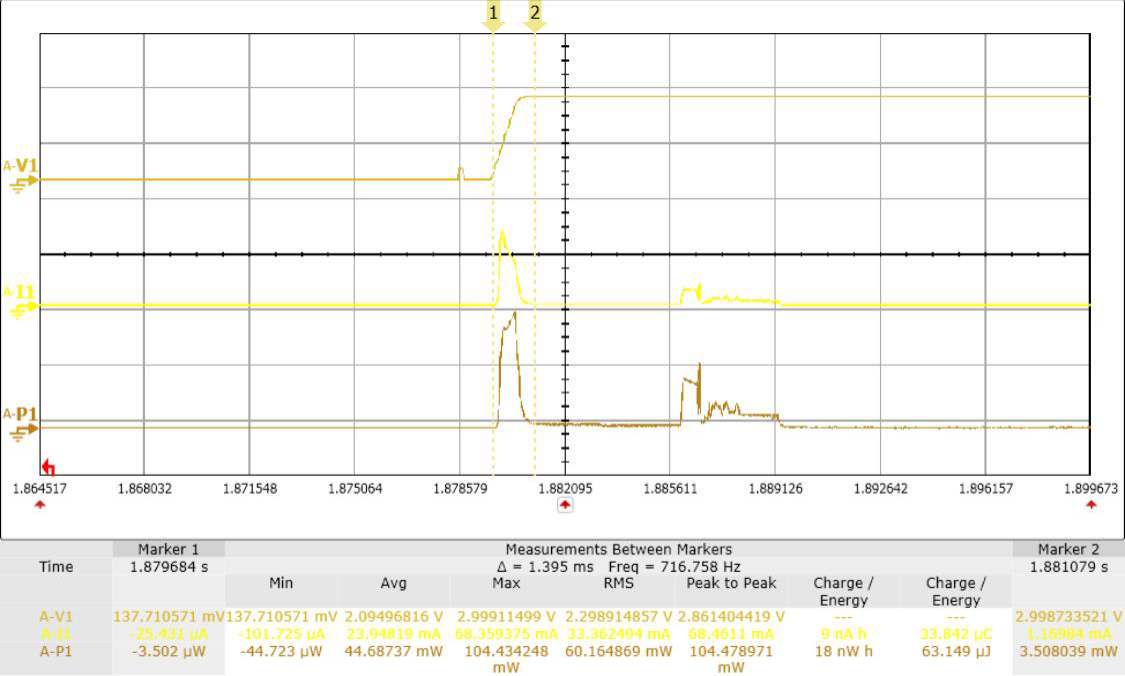
\includegraphics[width=1.0\textwidth] {3Vorgehen/imag/Energie_Laden_Kondensatoren_Sensortag.png}
  \caption{Aufladen Kondensatoren TI-SensorTag}
  \label{energie_kondensatoren_sensortag}
\end{figure} 
 
\begin{figure}[ht]
  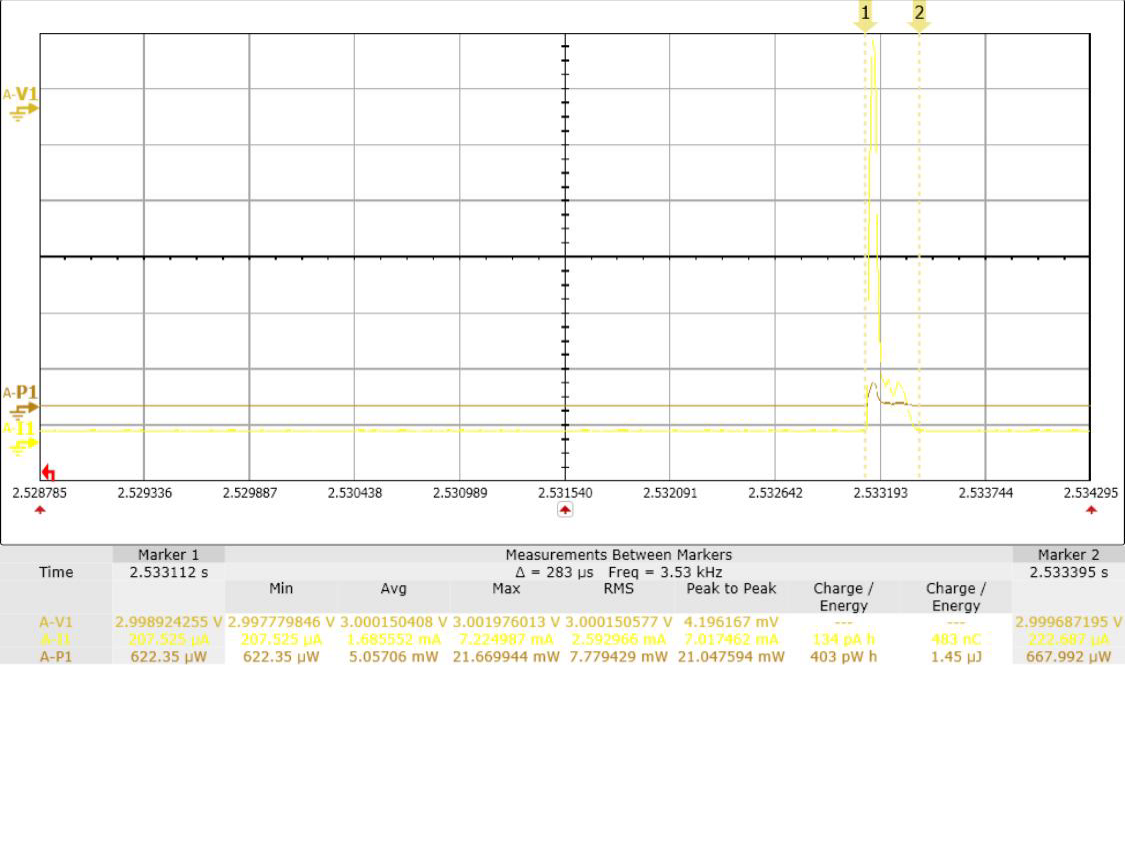
\includegraphics[width=1.0\textwidth]{3Vorgehen/imag/Refresh.png}
  \caption{Energie Refreshen}
  \label{energie_refresh}
\end{figure}

\begin{figure}[ht]
  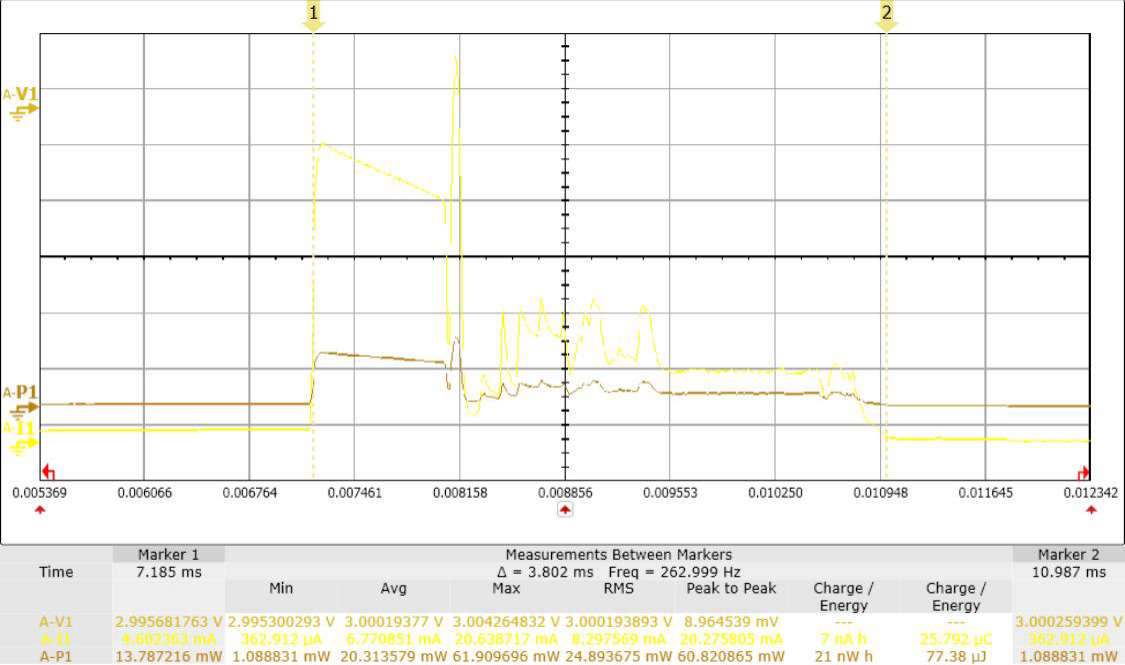
\includegraphics[width=1.0\textwidth]{3Vorgehen/imag/Init.png}
  \caption{Energieverbrauch für Initialisierung}
  \label{energie_init}
\end{figure}

\begin{figure}[ht]
  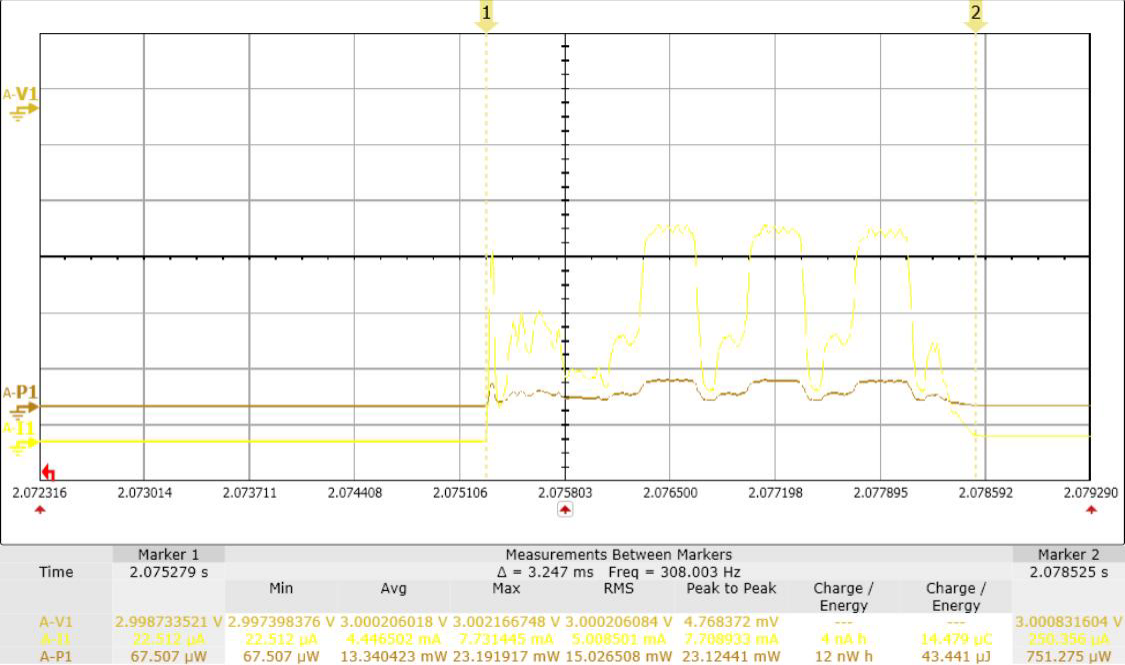
\includegraphics[width=1.0\textwidth]{3Vorgehen/imag/Senden.png}
  \caption{Energieverbrauch senden eines BLE-Paketes mit Sensordaten}
  \label{energie_senden}
\end{figure}

\clearpage
Die Initialisierung ist vergrössert in der Abbildung  \ref{energie_init} dargestellt. Im Überblick geht sie unter, da die Initialisierung direkt ans Laden der TI-SensorTag-Kondensatoren folgt. Da der Peak des Ladens viel höher ist, erscheinen die nachfolgenden Enerigeverbrauche nicht deutlich. Die Energiemessungen einzelner Stellen zeigen, dass für die Initialisierung 77.38 $\mu$J, für das Refreshen ca. $1.4\mu$J (Abbildung \ref{energie_refresh}) und für das Senden des BLE-Pakets (Abbildung \ref{energie_senden}) 43.44 $\mu$J verbraucht werden. Das Senden des BLE-Paketes ist bei der Zeitmarke 2.07 s.


\subsubsection*{Energieverbrauch Starten des Drucksensors}

Auf dem TI-SensorTag wird der Drucksensor BMP 208 von Bosch Sensortec verwendet. Bei der Zeitmarke 1.34 s wird der Sensor gestartet. Die Abbildung \ref{energie_drucksensor} dokumentiert einen Energieverbrauch von 5.753 $\mu$J zum Starten des Sensors.

\begin{figure}[ht]
  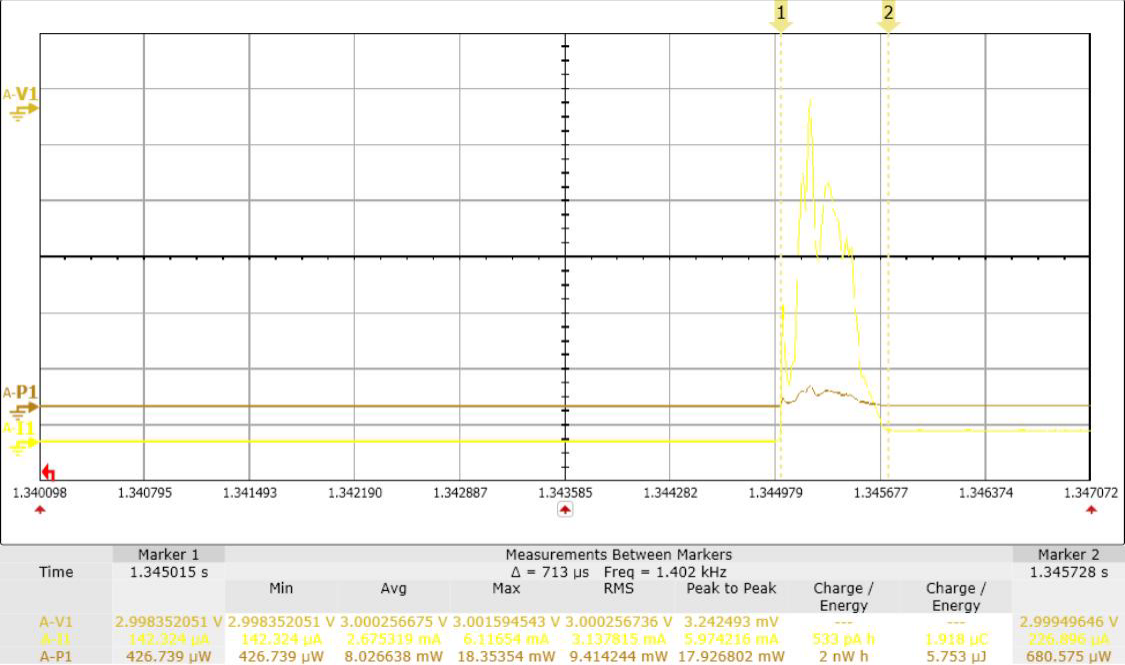
\includegraphics[width=1.0\textwidth]{3Vorgehen/imag/Drucksensor.png}
  \caption{Energieverbrauch des Drucksensors BMP 280}
  \label{energie_drucksensor}
\end{figure}

\clearpage

\subsubsection*{Energieverbrauch beim Starten des Temperatursensors}

Der Temperatursensor TMP0007 von Texas Instruments verbraucht für das Starten 10.635 $\mu$J. Dies findet bei der Zeitmarke t = 1.54 s statt.

\begin{figure}[ht]
  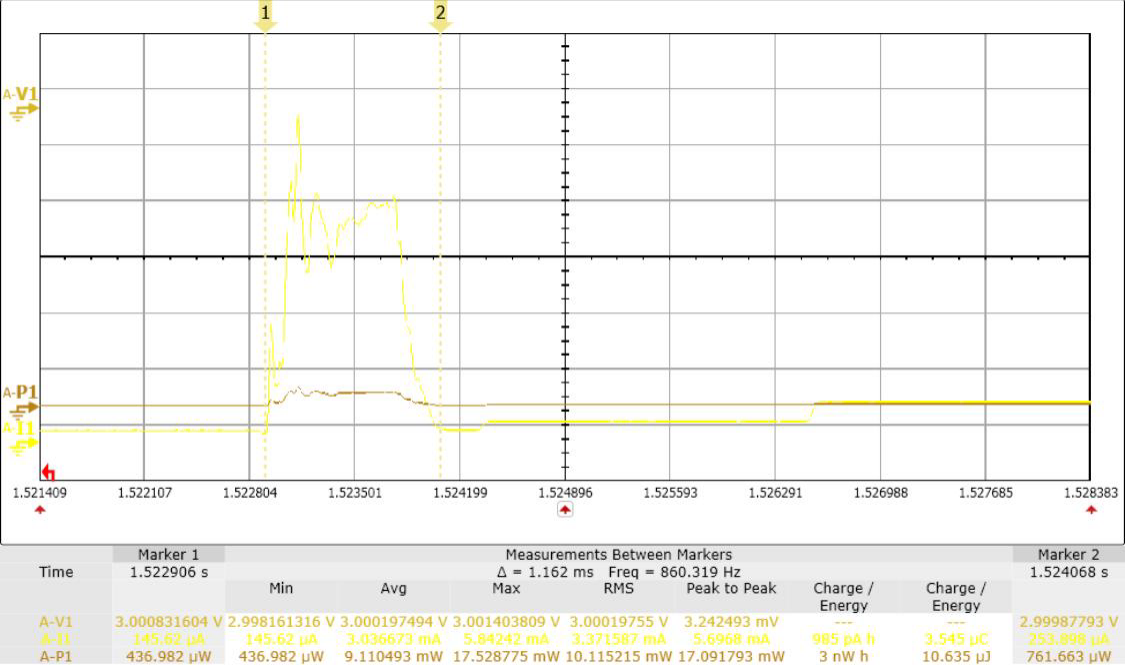
\includegraphics[width=0.7\textwidth]{3Vorgehen/imag/tempSensor.png}
  \caption{Energiemessung Temperatursensor auf TI-SensorTag}
  \label{energie_tempsensor}
\end{figure}

\subsubsection*{Energieverbrauch Feuchtigkeitssensor}

Der Feuchtigkeitssensor HDC1000 der Marke Texas Instruments verbraucht 6.358 $\mu$J, siehe Abbildung \ref{energie_humidity}.

\begin{figure}[ht]
  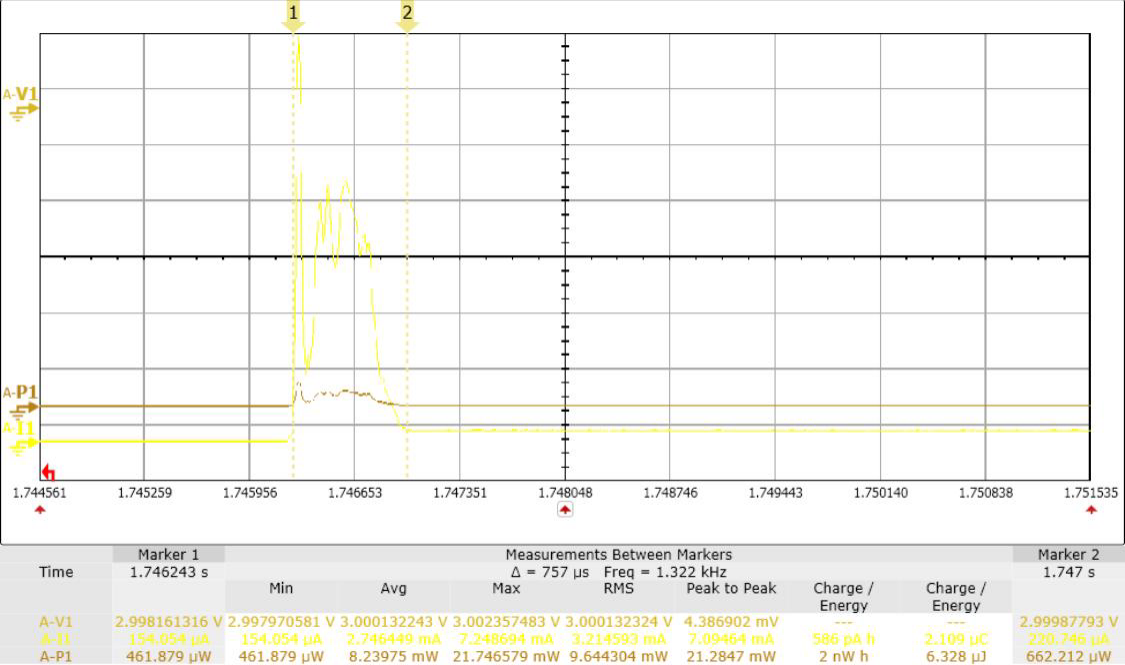
\includegraphics[width=0.7\textwidth]{3Vorgehen/imag/Humidity.png}
  \caption{Energieverbrauch Feuchtigkeitssensor}
  \label{energie_humidity}
\end{figure}

\enlargethispage*{15cm}

\clearpage
Um die verschiedenen Energiewerte in Bezug zueinander zustellen, werden in der Tabelle \ref{tab_zsm} die Energiewerte zusammengesfasst und in der Abbildung \ref{energie_zsm} der Verbrauch aller Aktionen in Bezug zueinander graphisch dargestellt. 


\begin{minipage}{\textwidth}
\captionof{table}{Zusammenfassung Energieverbrauch nach Aktion}
\label{tab_zsm}
\begin{tabbing}
    Aktion \hspace{6cm}                       \quad\= Energie \\[0.8ex]
    Laden C TI-Sensortag            \> 63 $\mu$J \\
    Initialisierung TI-Sensortag    \> 77 $\mu$J \\
    Refresh-Peaks während 10 s      \> 14 $\mu$J \\
    Starten Drucksensor             \> 6 $\mu$J \\
    Starten Temperatursensor        \> 11  $\mu$J \\
    Starten Feuchtigkeitssensor     \>  6 $\mu$J \\
    Senden BLE-Paket nur Geschwindigkeit\> 33 $\mu$J\\
    Senden BLE-Paket mit Sensordaten   \> 43 $\mu$J \\
\end{tabbing}
\end{minipage}

\begin{figure}[ht]
  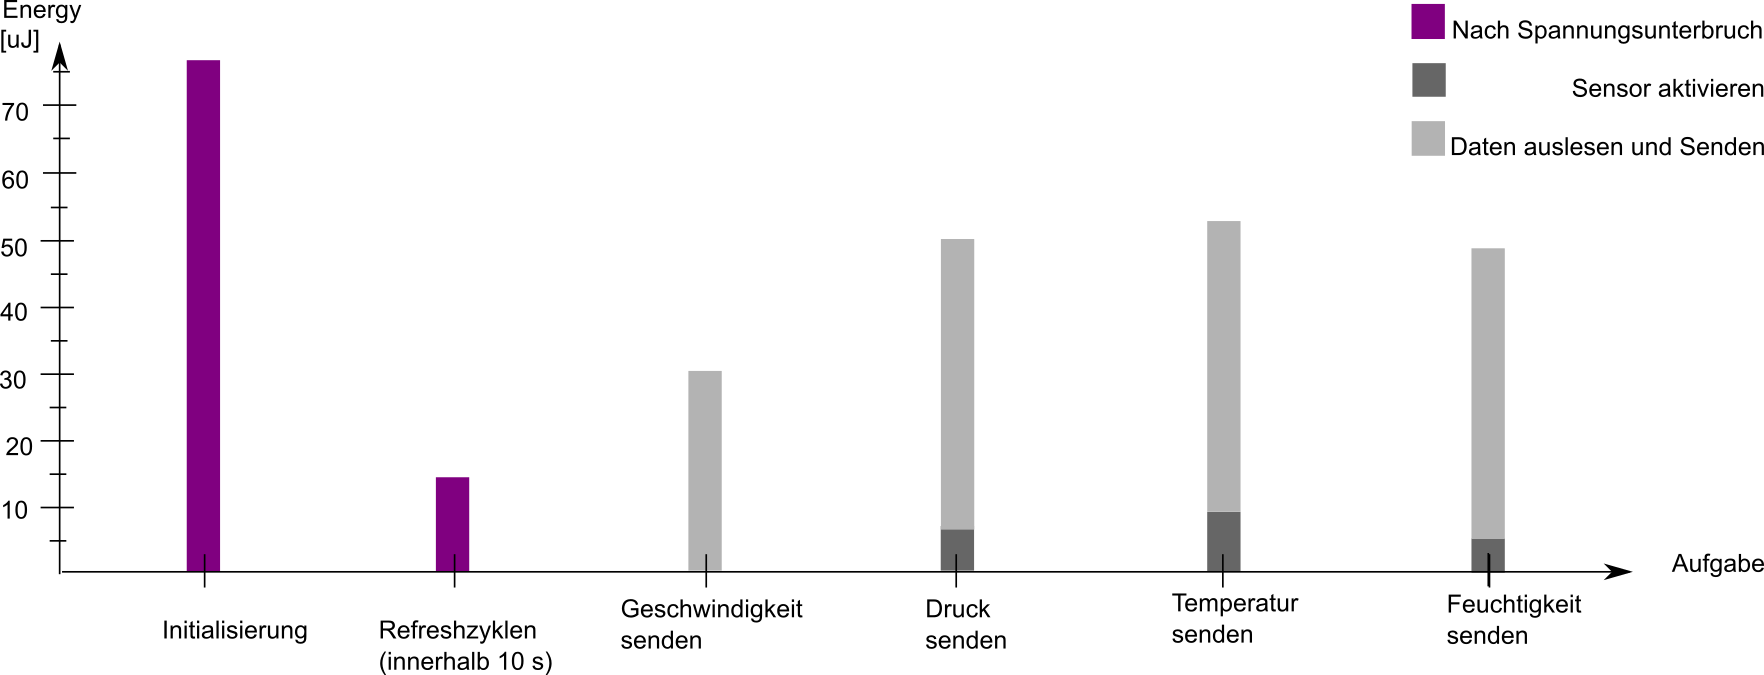
\includegraphics[width=1.0\textwidth]{3Vorgehen/imag/Energy_pro_Aufgabe.png}
  \caption{Energieverbrauch pro Aufgabe}
  \label{energie_zsm}
\end{figure}

Es wird deutlich, dass die Initialisierung und das notwendige Refreseshen des Speichers zusammen (die Balken sind violett)  fast gleich viel Energie brauchen, wie das Senden zweier BLE-Pakete mit Sensorwerten. Aus diesem Grund hat erste Priorität beim Power Management, dass die Speisung V\_SUP nicht abstellt. Denn wenn bei der Datenverarbeitung zu viel Energie verbraucht wird, fällt die Speisung aus. Jedes Mal wenn die Speisung unterbrochen wird, ist eine neue Initialisierung notwendig.


% x.2 ---------------------------------
\subsection{Energiekalkulation}
\label{v_e_kalkulation}

Die Energiekalkulation dient der Bestückung des Kondensators STS und der Definition von Schwellwerten für die Register im EM8500-Chip. Es wird vom schlechtesten  Fall, also einer Geschwindigkeit von 10 km/h, und dem noch nicht optimalen Energieverbrauch des TI-Sensortags V4 ausgegangen. Laut Datenblatt des EM8500 (\cite{datasheet_EM85}, S.\,9, Abschnitt Operating Conditions ) soll STS zwischen 10 - 100 $\mu$F gross sein. Typisch ist 47 $\mu$F. Die Grundlagen zur Energiekalkulation sind im Theorieteil \ref{th_energiebilanz} abgebildet. Als oberer Schwellwerte beim STS wird 3 V angenommen. Die Berechnung dazu findet sich in der Gleichung \ref{eq:bat_min_low_schwellwert}. 

\begin{flalign}\label{eq:e-high-e-low}
  E_{Applikation} &= E_{Laden C} + E_{Init} + E_{Refreshen}+ E_{Start Drucksensor} + E_{Senden BLE} \\\nonumber
       &= 63\, \mu J + 77\, \mu J + 14\, \mu J+ 6\, \mu J + 43\, \mu J = 203\, \mu J\nonumber
\end{flalign}

\begin{flalign}\label{eq:e_sts}
  C_{STS} &= \frac{2\times 203\, \mu J}{3^2 - (2.1)^2}\\
          &= \frac{ 406\, \mu J}{9 - 4.41}\\\nonumber
          &= \frac{ 406\, \mu J}{4.59}\\\nonumber
          &= 88.45\, \mu F
\end{flalign}

Der Wert wird aufgerundet auf 100 $\mu$F, um genügend Energie zu haben.

\subsubsection*{MPP einstellen}

Während der Entwicklung des Harvesters wurde die Leistungskurve aufgenommen (siehe Messprotokoll \cite{messung_harvester_finish}). Wie im Theorieteil \ref{harv_diff} erklärt unterscheidet sich das Leistungsmaximum nach Geschwindigkeit. Weil das Ziel ein funktionstüchtiger Prototyp bei 10 km/h ist, bezieht sich das Einstellen auf dieses Leistungsmaximum. Das Leistungsmaximum liegt beim entwickelten Bicycle Computer bei 24.77  $\mu$W. Die MPP-Ratio liegt beim MPP bei 47.16 \thinspace\% (siehe Messprotokoll \cite{messung_harvester_finish}). Die MPPT-Ratio liegt somit unter 50\thinspace\%. In der Umsetzung eines Energy Managements mit dem EM8500-Chip ergibt sich das Problem, dass nur Konfigurationen von MPPT-Ratios von 50 - 80\thinspace\% erlaubt sind (siehe Tabelle unten). Zudem sind die Einstellungsschritte der tieferen MPPT-Ratio von 50\thinspace\% bis 67\thinspace\% gröber als die von 71\thinspace\% bis 88\thinspace\%. Dies, weil der EM8500-Chip für Harvester vom Typ TEG (MPPT-Ratio 50\thinspace\%) und Solarzellen konzipiert ist. Bei der Bewegungsinduktion ist dieser vorgegebene Range nicht ideal.

\clearpage
\begin{minipage}{\textwidth}
    \captionof{table}{MPPT-Ratio Einstellungen EM8500}
    \begin{tabbing}
    Registerwert   \quad\= MPPT-Ratio    \\[0.8ex]
    0x00           \> 50\thinspace\% \\
    0x01           \> 60\thinspace\%\\
    0x02           \> 67\thinspace\%\\
    0x03           \> 71\thinspace\%\\
    0x04           \> 75\thinspace\%\\
    0x05           \> 78\thinspace\%\\
    0x06           \> 80\thinspace\% \\
    0x07           \> 82\thinspace\%\\
    0x08           \> 83\thinspace\%\\
    0x09           \> 85\thinspace\%\\
    0x0A           \> 86\thinspace\% \\
    0x0B           \> 87\thinspace\%\\
    0x0C           \> 88\thinspace\%\\
    \end{tabbing}
\end{minipage}


% x.3 -------------------------------------
\subsection{Einstellen der Schwellwerte}
\label{v_schwellwerte}

Das Konzept der Schwellwerte von VSTS und VLTS sind im Theorieteil bei der Erklärung des Speicherkonzepts des EM8500-Chips im Unterkapitel \ref{speicher_konzept} beschrieben. Das Ziel ist, dass sich LTS bei 10 km/h entlädt. Die Berechnung der Schwellwerte stammt aus dem Theorieteil \ref{th_energiebilanz}.

Aus der Vorgängerarbeit sind in der Tabelle unten notierte Konfigurationswerte überliefert. Bei der Inbetriebnahme fiel der hohe Schwellwert von STS\_LOW (3.6 V) auf, ab der erst die Applikation gespiesen wird. Der hohe Wert beruht auf dem Versuch, möglichst viel Energie vor dem Datensenden zu sammeln. Ein hoher Schnellwert verzögert die Zeit bis zum ersten Datensenden. Die Vorgänger wählten in ihren Einstellungen eine MPPT-Ratio von 88\thinspace\%.

\begin{minipage}{\textwidth}
    \captionof{table}{Konfiguration Vorgängermodell}
    \begin{tabbing}
    Register \hspace{4cm} \quad\= Wert \\[0.8ex]
    v\_bat\_max\_hi       \> 4.2 V \\
    v\_bat\_max\_lo       \> 4.1 V \\
    v\_bat\_min\_hi\_dis  \> 3.6 V \\
    v\_bat\_min\_hi\_con  \> 2.1 V \\
    v\_bat\_min\_lo       \> 1.8 V \\
    v\_appl\_max\_hi      \> 3.8 V \\\
    v\_appl\_max\_lo      \> 3.7 V \\ 
    mppt\_ratio            \> 88\thinspace\% \\
    \end{tabbing}
\end{minipage}

Nach der Energiemessungen der Version V3 des TI-SensorTags (siehe \cite{messung_energie_sensortag}), in dem die Geschwindigkeit per BLE gesendet werden kann, entstanden folgende Schwellwerte:

\begin{minipage}{\textwidth}
    \captionof{table}{Konfiguration aufgrund Geschwindigkeitsmessung}
    \begin{tabbing}
    Register\hspace{4cm} \quad\= Wert \\[0.8ex]
    v\_bat\_max\_hi       \> 4.8 V \\
    v\_bat\_max\_lo       \> 4.7 V \\
    v\_bat\_min\_hi\_dis  \> 2.8 V (siehe Berechnungen unten)\\
    v\_bat\_min\_hi\_con  \> 2.1 V \\
    v\_bat\_min\_lo       \> 2.0 V (vorgegeben von TI-SensorTag)\\
    v\_appl\_max\_hi      \> 3.8 V \\\
    v\_appl\_max\_lo      \> 3.7 V \\ 
    mppt\_ratio            \> 50\thinspace\% (aus MPP-Kurve Harvester)\\
    \end{tabbing}
\end{minipage}

Die Grundlage bildete die Gleichung  $E_{Applikation}= E_{STS\_HIGH} - E_{STS\_LOW}$, wobei  $E_{Applikation}$ aus der Messung von V4 mit total 189 $\mu$J für die Initialisierung und das Senden der Daten gebraucht werden. Als Kondensatorwert für STS wird 100 $\mu$F genommen. So ergibt sich folgender minimaler oberer Schwellwert:

\begin{flalign}\label{eq:bat_min_low_schwellwert}
    (v\_bat\_min\_low) ^2  &=  \frac{2\, \times \, E_{Applikation}}{C_{STS}} + (V_{STS\_LOW})^2\\
     &=  \frac{2\, \times \, 189\, \mu J}{100 \,\mu F} + (2.0\, V)^2\\ \nonumber
    v\_bat\_min\_low  &=  \sqrt{\frac{378 \,\mu J}{100 \,\mu F} + 4\, V^2} = \sqrt{7.8\, V^2} = 2.79 \,V \\\nonumber
\end{flalign}

Wichtigster Wert in der Konfiguration ist jedoch der korrekte MPPT-Wert. Er wird auf das Minimum (50\thinspace\%) gesetzt. Das Maximum des Ladezustands  wird auf den maximal erlaubten Wert gesetzt: v\_bat\_max  = 4.8 V bzw. 4.7 V. Denn solange Energie geerntet werden kann, soll sie gespeichert werden. v\_appl\_max spielt in unserer Anwendung keine wichtige Rolle. Der Wert wird von den Vorgängern übernommen.

Das Zusammensetzen der Last (TI-SensorTag) mit der konfigurierten Hardware erstaunte. Ab 25 km/h funktionierte die Schaltung gut. Doch darunter reagiert der EM8500-Chip nicht. Weder STS noch LTS konnten sich laden. Nachmessungen am Eingang vom EM8500-Chip ergaben, dass bei  10 km/h und einer MPPT-Ratio von 50\thinspace\% eine Spannung von 0.2 V anliegt. Diese ist zu tief, um den Booster zu starten. Erst bei höherer Geschwindigkeit wird eine Eingangsspannung von mehr als 0.3 V erreicht und das System beginnt zu funktionieren. Um eine Minimalspannung von 0.3 V bei niedrigen Geschwindigkeit zu garantieren wird die MPPT-Ratio zukünftig auf den zweittiefsten Wert (60 \thinspace\%) eingestellt.

Ein unerwartetes Verhalten des Drucksensors zeigt sich bei der Implementation des Auslesens. Der BLE-Sniffer empfängt die Druckdaten korrekt, doch beim Anschliessen des TI-SensorTags an die Harvesterschaltung, riss die Spannung sofort zusammen. Innert kürzester Zeit entlädt sich der STS sowie der parallel geschaltene LTS. Unterschreitet der STS den Schwellwert von 2 V, so stellt die Speisung der Applikation ab (siehe im Unterkapitel 3.4.1 Abbildung im Abschnitt \ref{erst_EMessungen}). Das Ausmessen des Energieverbrauchs bringt Klarheit: Die I2C-Kommunikation und das Aufstarten des Sensors brauchen mehr Energie als das Berechnen der Geschwindigkeit aus den Reed-Switch Impulsen (siehe Abbildung \ref{r_bild_e_zusammenfassung} im Resultat-Teil).


Durch den deutlich höheren Energieverbrauch wird eine Power-Optimierung im Softwareteil notwendig. Es zwingt aber auch dazu, den Schwellwert von STS\_LOW  wieder zu erhöhen. Die finale Konfiguration ist im Resultate-Teil abgebildet.


% x.4 -----------------------------------------
\subsection{Energiezustand des Systems}
\label{v_energiezustand}

Die letzte der vier Aufgaben aus der Optimierungsliste nach der Inbetriebnahme (siehe Unterkapitel \ref{optimierung}) ist das variable Anpassen des BLE-Paketsendens aufgrund des Energiezustandes. Im ersten Unterkapitel wird das Einteilen des Systems in Energiezustände beschrieben. 

\subsubsection*{Definition von Energiezuständen}
\label{def_zustaende} 

Da die produzierte Energie von der Fahrgeschwindigkeit abhängt, werden die Energiezustände aufgrund der Fahrgeschwindigkeit definiert. Welche Aufgaben in welchem Energiezustand erledigt werden, folgt in den Abbildungen \ref{LOW_ENER}, \ref{MID_ENER} und \ref{HIGH_ENER}, direkt nach der Definition der Zustände. 

\begin{minipage}{\textwidth}
    \captionof{table}{Energiezustände aufgrund der Geschwindigkeit}
    \begin{tabbing}
       Geschwindigkeit\quad\= Systemzustand\\[0.8ex]
       0 - 15 km/h        \> LOW\_ENERGY\\
       15 - 20 km/h       \> MIDDLE\_ENERGY\\
       ab 20 km/h         \> HIGH\_ENERGY\\    
    \end{tabbing}
\end{minipage}

Bei wenig Energie lädt sich nur der STS. Erreicht er den Schwellwert für die Speisung der Applikation, so erhält TI-SensorTag Spannung. Die Reed-Impulse werden ausgelesen, der zweite Prozessor für das Senden der BLE-Pakete gestartet und die Daten übertragen. Bei wenig Energie verbrauchen diese drei Aktionen sämtliche zur Verfügung stehende Energie. Denn LTS hat sich nicht geladen. Die Energie genügt nicht für weitere Aktionen.

\begin{figure}[ht]
    \begin{minipage}[t]{0.5\textwidth}
      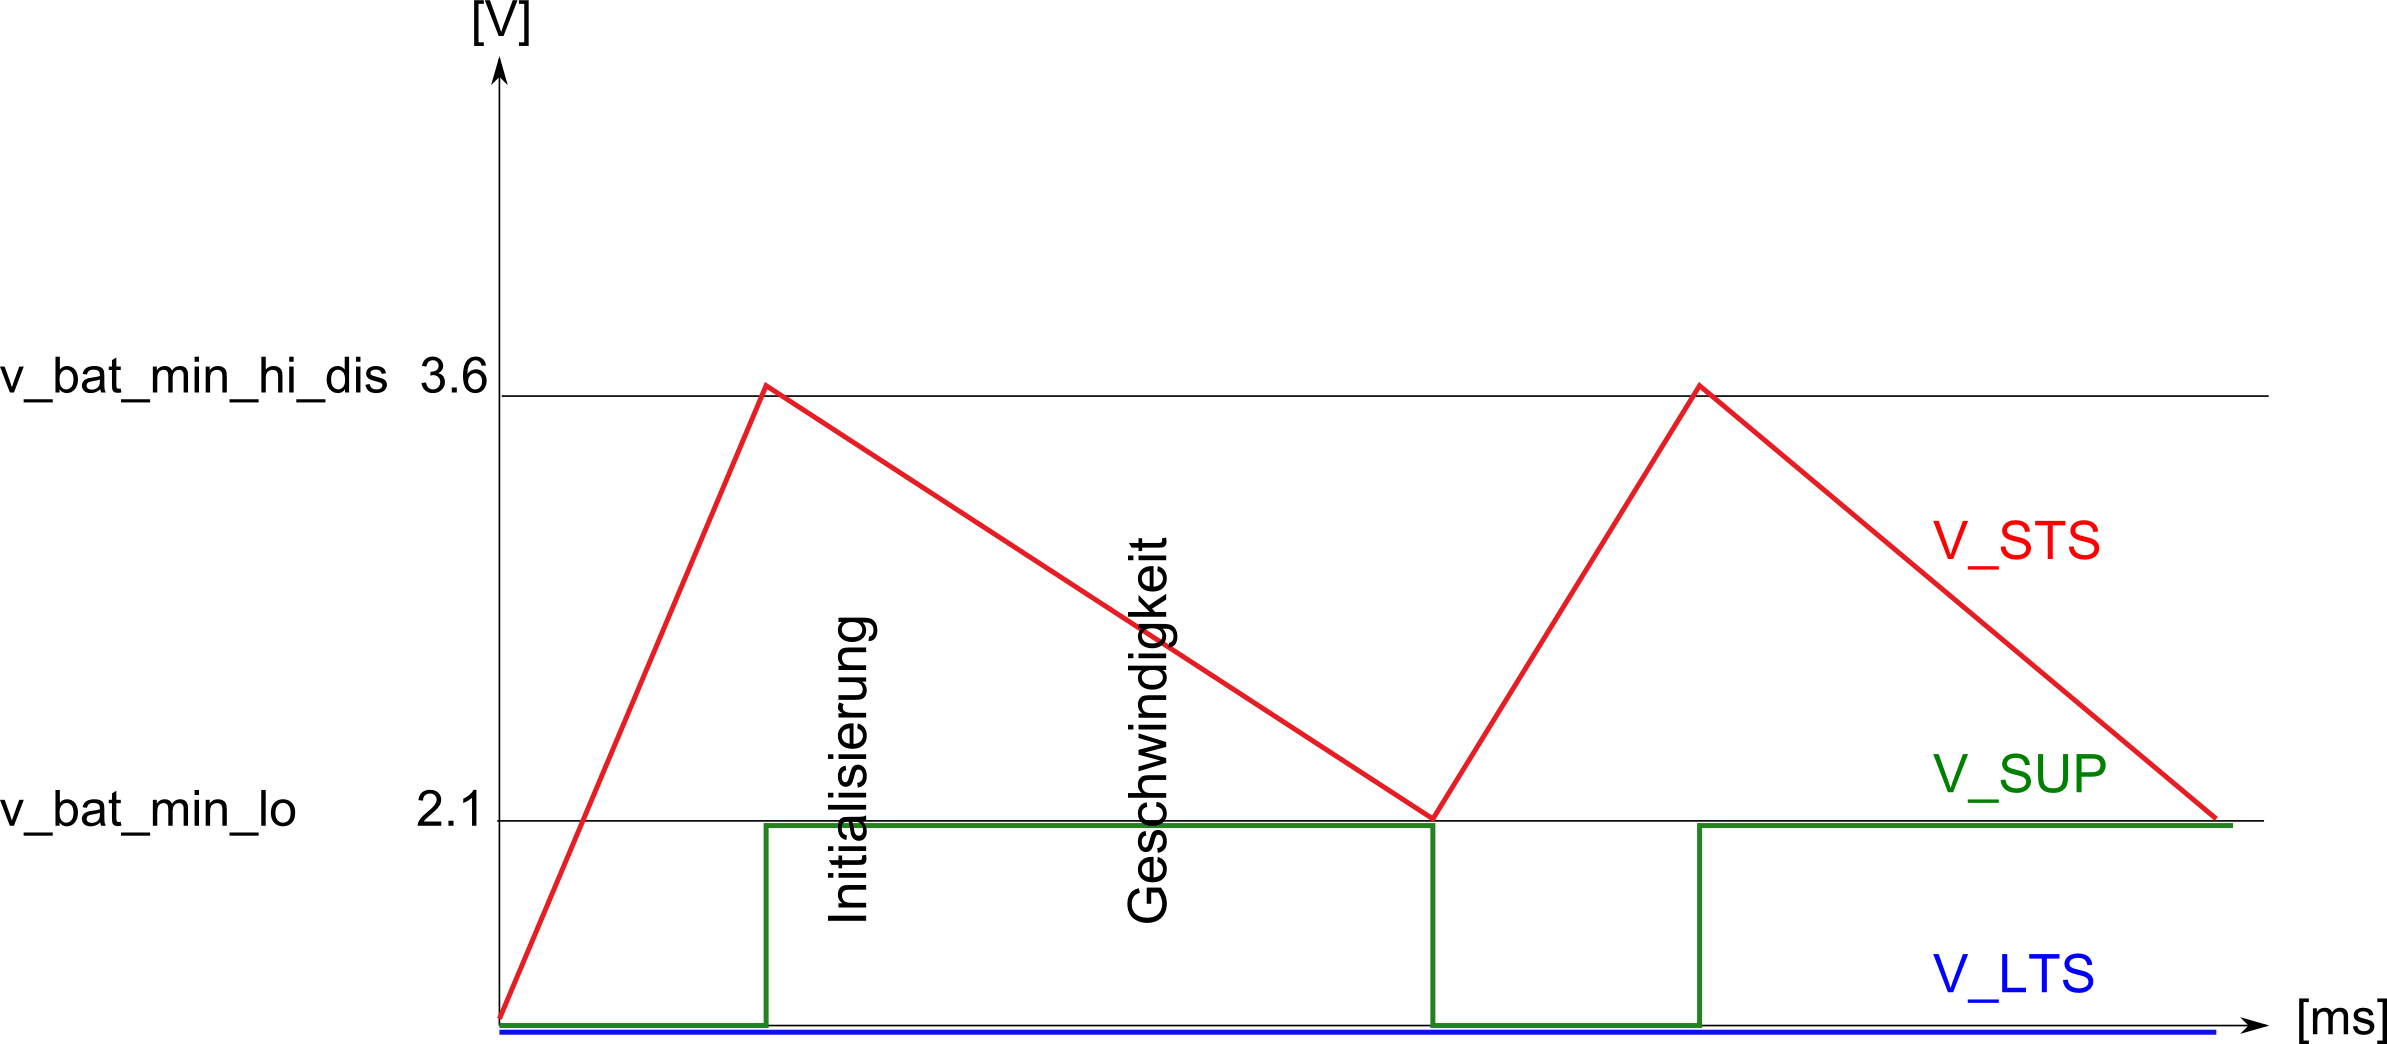
\includegraphics[width=1.0\textwidth]{3Vorgehen/imag/LOW_ENERGY.png}
      \caption{Wenig Energie}
      \label{LOW_ENER}
    \end{minipage}
    \begin{minipage}[t]{0.5\textwidth}
      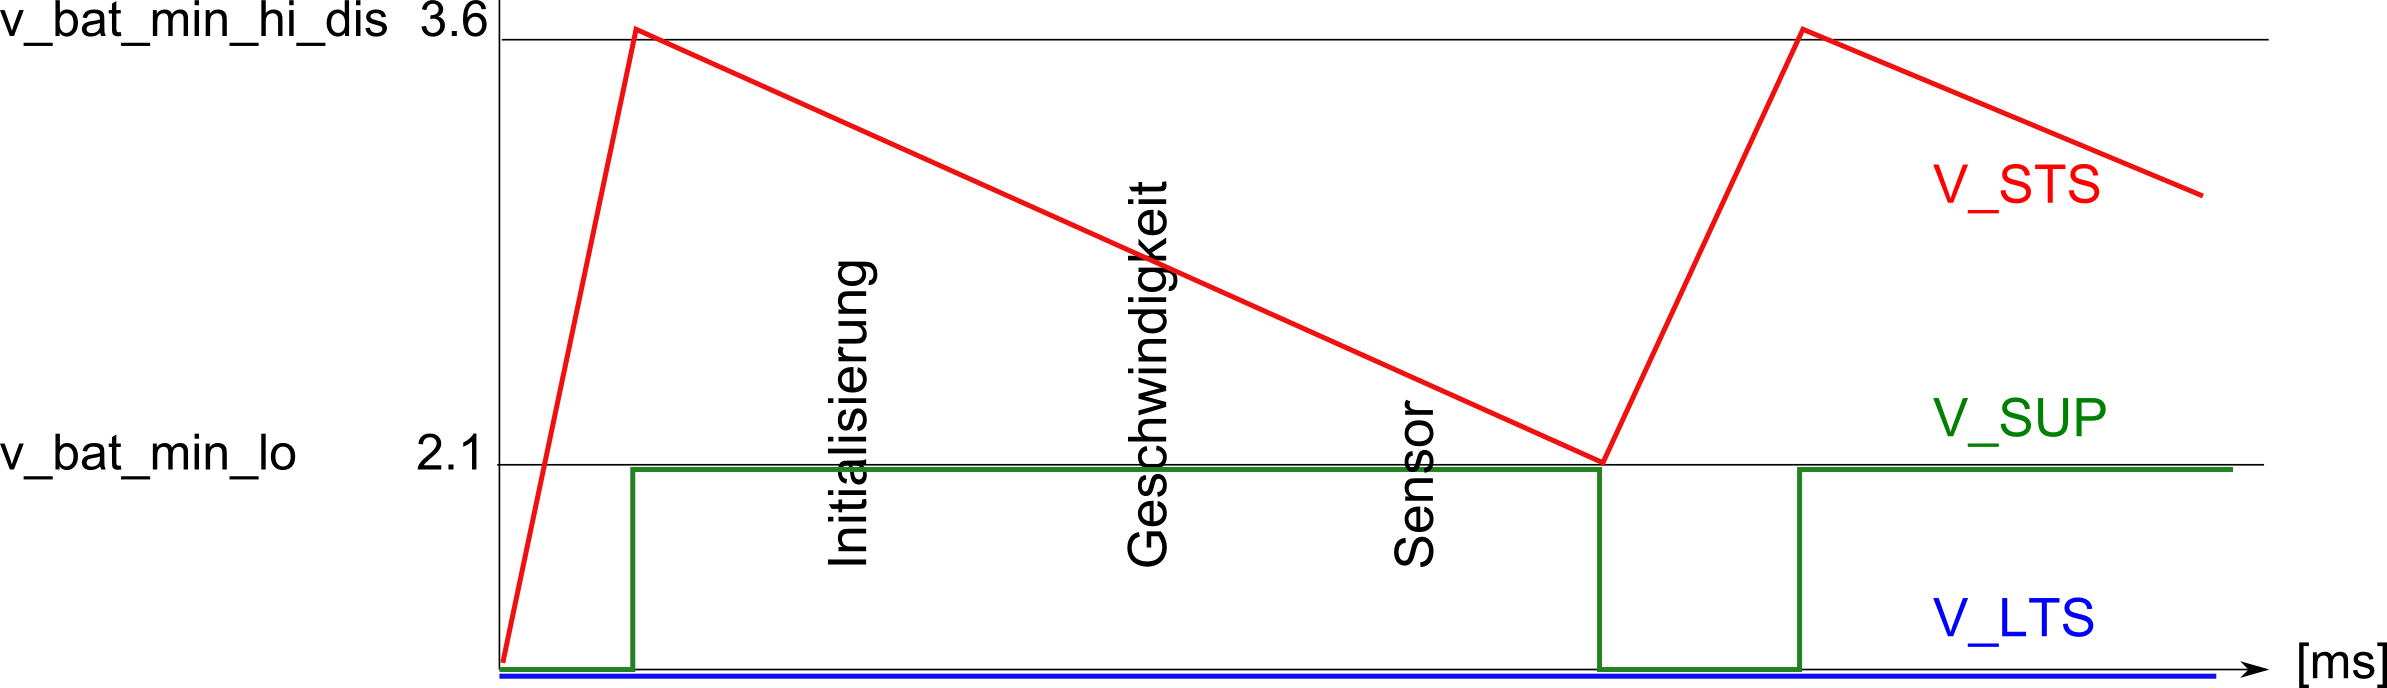
\includegraphics[width=1.0\textwidth]{3Vorgehen/imag/MIDDLE_ENERGY.png}
      \caption{Mittlere Energie}
      \label{MID_ENER}
    \end{minipage}
\end{figure}

Bei etwas mehr Energie befindet sich das System in einem Zwischenzustand (Abbildung \ref{MID_ENER}). Zu jeder Geschwindigkeitsmessung wird ein Sensor ausgelesen. Im Idealfall unterstützt LTS die Stabilität. Wenn nicht, schaltet V\_SUP bei zu wenig Energie ab. Im hohen Energiezustand werden mit jedem Geschwindigkeitspaket die aktualisierten Werte der drei Sensoren mitübertragen. 

\begin{figure}[ht]
  \includegraphics[width=1\textwidth]{3Vorgehen/imag/HIGH_ENERGY_2.png}
  \caption{Viel Energie}
  \label{HIGH_ENER}
\end{figure}


% 4 ---------------------------------------------------------------------------
\section{Power Management}
\label{powerOptimierung}

Das Power Management wird mit dem TI-SensorTag umgesetzt. Im ersten Unterkapitel \ref{keinROTS} wird beschrieben, auf welche Bibliotheken und Hilfen man von Texas Instruments zurückgreifen kann. In nächsten Unterkapitel \ref{PowerDomains} werden die Power-Domains des TI-SensorTags erklärt und im letzten Unterkapitel die Umsetzung, z.B. wie Schlafenszeiten eingebaut werden \ref{sleep_funktion}.


\subsection{Programmieren für Low-Power-Applikation im Adevertising Mode}
\label{keinROTS}

Das ausgewählte TI-SensorTag ist für Low-Power-Anwendungen ausgelegt. Die Low-Power-Programmbeispiele von TI basieren auf dem TI-Real Time Operating System (kurz RTOS). Da bei 10 km/h Energie im $\mu$J-Bereich zur Verfügung steht, läuft die Applikation im Advertising Mode. Dieser braucht weniger Energie als der Connected Mode und der Overhead eines Betriebsystems (RTOS) und der Initialisierung des BLE-Stacks sind nicht notwendig. Der Nachteil dieser schlanken Programmierung ist, dass die TI-SensorTag Beispiele ausschliesslich auf RTOS aufbauen, und somit nicht 1:1 übernommen werden können. Für nachkommende Entwicklerinnen und Entwickler sind zwei Vorzüge und zwei Nachteile dieser Wahl festgehalten:

\begin{minipage}{1\textwidth}
    \begin{enumerate}
        \item Vorteil ohne RTOS: Ein sehr schlanker Code entsteht. Die Register werden direkt gesetzt, und die Funktionsaufrufe sind sehr schnell.
        \item Vorteil ohne RTOS: Man muss sich nicht in das TI-RTOS-Konzept einarbeiten. Die Message-Queue und das Thread-Handling bei TI muss man nicht kennen.
        \item Nachteil ohne RTOS: TI implementierte über die Library die Hauptaktivitäten wie Power Domains einschalten oder Kommunikation zu Peripheriegeräten aufbauen. Die Zugriffe werden vom OS übernommen. Ohne RTOS muss man sich selber z.B. ums Aufwachen oder das Abhandeln der Interrupts kümmern.        
       \item Nachteil ohne RTOS: Eine Dokumentation zur umfangreichen Library (cc26xxware/driverLib) fehlt, da TI davon ausgeht, dass man über das OS auf die Bibliothek zugreift. Die internen Abhängigkeiten zu verstehen, ist nicht einfach. Unerwünschte Nebeneffekte treten auf.
    \end{enumerate}
\end{minipage}

\subsection{Power Domains beim TI-SensorTag}
\label{PowerDomains}

Bei einer Low-Power-Applikation hat das Ein- und Ausschalten von sogenannten Power Domains eine zentrale Rolle. Das TI-SensorTag unterscheidet 10 Power Domains. Ein Überblick  ist in der Abbildung  \ref{supply_syst} abgebildet. Das Konzept der Verbrauchsoptimierung besteht im Abschalten unnötiger Peripherie- und Prozessorteilen. Nur absolut notwendige Power Domains laufen weiter. Der Teil, der nicht abstellt wird, wird AON (Always On) genannt. Zu dieser Domain gehört ein Clock, ein Timer, gewisse Interrupts und Schnittstellen. Im Anhang \ref{anhang_sensortag_PowerDomain} ist in der Abbildung \ref{a_powerdomain} detailliert dargestellt, wie die einzelnen Power Domains sich beim Ausschalten verhalten. So werden z.B. für das RAM und die GPIO Refreshzyklen benötigt. Beim RAM bedeutet dies eine Speicherauffrischung, bei der GPIO eine Kontrolle der Pinzustände.

\clearpage
\begin{figure}[ht]
  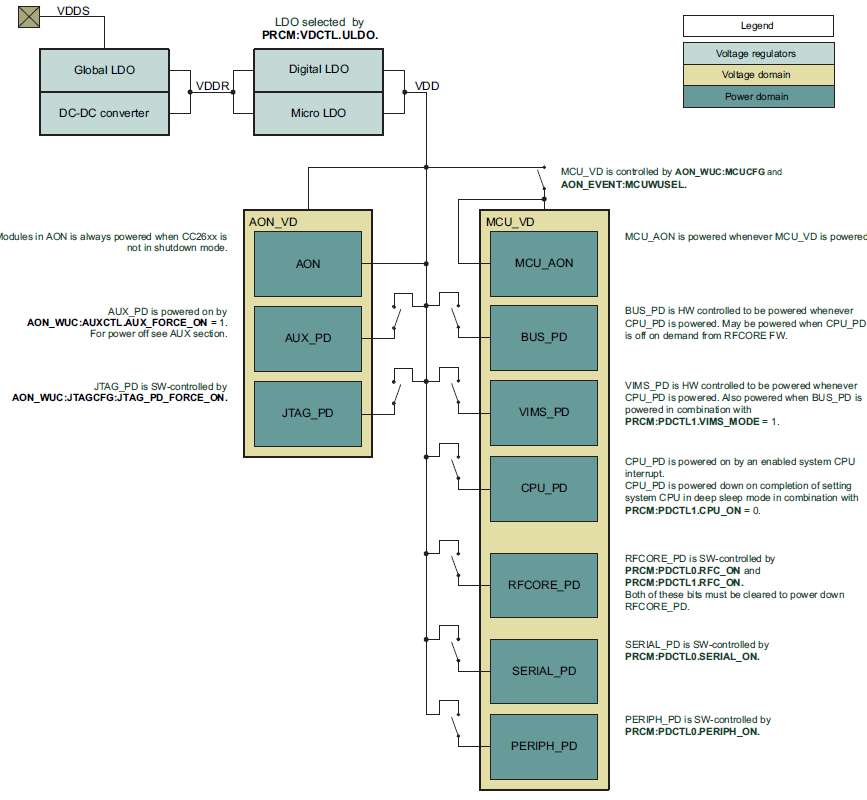
\includegraphics[width=1.0\textwidth]{3Vorgehen/imag/powerdomain_1.png}
  \caption{Supply System TI-SensorTag aus: \cite{Sensortag_Manual}, S.\,416}
  \label{supply_syst}
\end{figure}


\subsection{Schlafenszeiten implementieren}
\label{sleep_funktion}

In der Theorie \ref{pm_sleep} wird das Schlafen zwischen Funktionsblöcken beschrieben. Der Energy-Management-Teil fasst zusammen, welche Aktionen bei welcher Energie gemacht werden können (siehe Abbildungen \ref{warten_zw_bloecken}). Das Auslesen der Sensoren ist nur möglich, weil die Aktionsblöcke aufgeteilt werden und das System dazwischen Schlafen geht. Die Abbildung \ref{warten_zw_bloecken} zeigt den implementierten Codeablauf der TI-SensorTag Version V4, bei einer Geschwindikeit unter 50 km/h. Der Fall von einer Geschwindigkeit von über 50 km/h, bei der V\_SUP nicht mehr abstellt, ist im letzten Unterkapitel illustriert.\\

\begin{figure}[ht]
  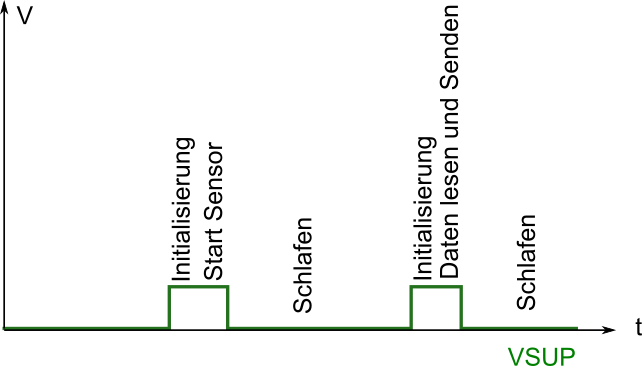
\includegraphics[width=0.5\textwidth]{3Vorgehen/imag/schlafen_funktionen.png}
  \caption{Schlafenszeiten zwischen Aktionen}
  \label{warten_zw_bloecken}
\end{figure}

Ist eine Aufgabe getätigt, wie z. B. das Starten eines Sensors, kann das System schlafen gehen. Dieses Prozedere funktioniert einwandfrei und sicher. Das System wacht aufgrund eines Interrupts wieder auf. Nachfolgend sind die zwei Hauptfunktionen: Vorbereiten zum Standby und ausschalten des Hauptprozessor abgebildet.

\subsubsection{Standby-Prozedur}
\label{vorbereiten}

Die abgebildete Funktion verdeutlicht exemplarisch, welche Schritte bei einer Programmierung ohne RTOS durch die Programmiererin bzw. den Programmierer ausgeführt werden.  Zum Verständnis werden einige Zeilen des Codes kurz kommentiert:\\ 

Zeile 2:\hspace{1cm}   Der Crystal-Oszillator wird abgeschaltet.\\
Zeile 3:\hspace{1cm}   Das Radio-Modul ebenfalls.\\ 
Zeile 4:\hspace{1cm}   Ein niedriger Takt wird eingestellt.\\ 
Zeile 5:\hspace{1cm}   Unnötige Peripheriespeisung wird abgestellt.\\ 
Zeile 6:\hspace{1cm}   Dem Prozessor wird erlaubt, seine Register zu refreshen und\\ 
Zeile 7:\hspace{1cm}   das Cache wird abgeschaltet.\\ 
Zeile 8:\hspace{1cm}   Der Refreshzyklus wird aktiviert.\\
Zeile 11:\hspace{1cm}  Das Intervall zwischen den Refreshzyklen wird berechnet.\\
Zeile 12:\hspace{1cm}  Es wird gewartet, bis alle Anweisungen abgeschlossen sind.\\



\begin{minipage}[t]{1\textwidth}
\small\begin{verbatim}
1    void go_to_standby(){ 
2        powerDisableXtal();
3        powerDisableRFC();
4        OSCHfSourceSwitch(); // activates lower clock
5        powerDisableAuxForceOn();
6        powerEnableMcuPdReq();
7        powerDisableCache();
8        powerDisableCacheRetention();
9
10        // calculate next recharge time
11        SysCtrlSetRechargeBeforePowerDown(XOSC_IN_HIGH_POWER_MODE);
12        SysCtrlAonSync();
13    } 
    \end{verbatim}\normalsize
\end{minipage} 	    

\clearpage
\subsubsection{Abschalt-Prozedur}
\label{ausschalten}

Nach der Vorbereitung zum Abschalten wird der Prozessor zum Schlafen geschickt.\\

Zeile 2:\hspace{1cm}   Cortex M3 wird zum Schlafen geschickt.\\
Zeile 3:\hspace{1cm}   Das Power-Control-Register erhält das Sleep-Flag.\\
Zeile 4:\hspace{1cm}   Die Always-On-Power-Domain muss die Konfigurationen speichern.\\
Zeile 5:\hspace{1cm}   Den Refrehzyklus-Wert setzen.\\
Zeile 6:\hspace{1cm}   Warten, dass alle Prozesse fertig abgehandelt sind.\\

\begin{minipage}[t]{1\textwidth}
\small\begin{verbatim}
1    void go_to_deep_sleep(){ 
2        powerDisableCPU();
3        PRCMDeepSleep();
4        SysCtrlAonUpdate();
5        SysCtrlAdjustRechargeAfterPowerDown();
6        SysCtrlAonSync();
7    }
\end{verbatim}\normalsize
\end{minipage}

\subsubsection{Sleep-Time-Übersicht bei Version V4}
	    
Bei den ersten Messungen der Sensoren riss V\_SUP so schnell zusammen, dass kein BLE-Paket gesendet werden konnte. Das Senden wird möglich, indem zwischen einzelnen Aufgaben geschlafen wird. Denn während dem das TI-SensorTag nur die minimale Energie verbraucht, kann der Bicycle Computer Energie sammeln. Während der Schlafenszeit steigt der Spannungswert an den Kondensatoren STS und LTS. Die Abbildung \ref{schnarch} zeigt, dass bei der Version V4 (siehe Messprotokoll \cite{messung_energie_sensortag}) die Aufgaben aufgeteilt werden. Dies entspricht dem Konzept des vorangehenden Unterkapitels mit der Abbildung \ref{warten_zw_bloecken}, nur dass in Abbildung \ref{schnarch} der Fall von einer Geschwindigkeit von über 40 km/h gezeigt wird, und V\_SUP deshalb nicht abstellt.\\   

Beim Senden von Sensordaten sind zwei Funktionen kritisch: das Starten eines Sensors und das Senden der Daten. Diese zwei Aufgaben werden getrennt und dazwischen geht das System schlafen (siehe vereinfacht dargestellt in der Abbildung \ref{schnarch}).\\

\begin{figure}[ht]
  \includegraphics[width=1.0\textwidth]{3Vorgehen/imag/HIGH_ENERGY_2.png}
  \caption{Auftrennen der Arbeit durch Schlafen dazwischen}
  \label{schnarch}
\end{figure}

Die Schlafenszeit wird experimentell ermittelt. Innerhalb des GPIO-Handlers zählt ein Counter die Reed-Switch-Interrupts, also die Radumdrehungen. Da am Fahrrad zwei Magnete befestigt sind, entspricht der Counterwert der doppelten Anzahl Radumdrehungen. Ist  das Zählermaximum erreicht, wird der Code rund um eine energiestarke Aktion ausgeführt. Danach geht das System schlafen. Das System soll so lang schlafen, dass die Spannung von V\_STS genug gross ist, dass die energiestarke Aktion ausgeführt werden kann. In der unten aufgeführten Tabelle findet sich eine grobe Count-Statistik der Version V4 für verschiedene Geschwindigkeiten. 

\begin{minipage}{\textwidth}
    \captionof{table}{Zählerstände für Schlafenszeit}
    \begin{tabbing}
   Geschwindigkeit \quad\= Counter-Wert  \quad\= Ladezeit STS    \quad\= Radumdrehungen\\[0.8ex]
   13 - 16 km/h          \> 100               \> 80 s    \> 50\\
   20 km/h               \> 50                \> 17 s    \> 25\\
   31 - 32 km/h          \> 50                \> 11 s    \> 25\\    
    \end{tabbing}
\end{minipage}

Das Setzen der Schlafenszeit ist einer globalen Variable gespeichert. Abhängig von der Geschwindigkeit, wird das Schlafensintervall (das Counter-Maximum) angepasst.






% 5 ---------------------------------------------------------------------------
\section{Applikationsentwicklung}

Nachfolgend wird der Aufbau von TI-SensorTag zusammen mit unserem selbst entwickelten Board als Sensor benannt und die Android-Applikation auf dem Smartphone wird einfach als Applikation benannt.

\subsection{Aufbau der Applikation}

\begin{figure}[ht]
    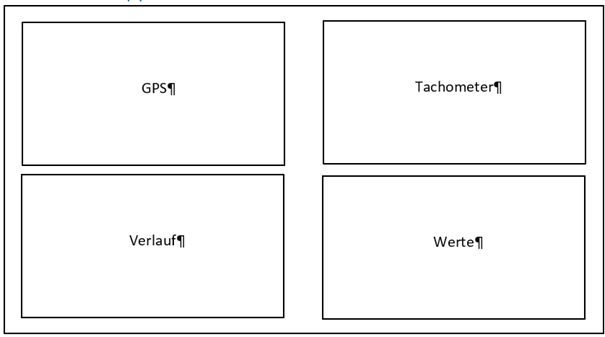
\includegraphics[width=0.5\textwidth]{3Vorgehen/imag/Aufbau_Applikation_erste_Version.png}
    \caption{Aufteilung des Bildschirms}\label{aufbau_applikation_1} 
\end{figure}

Der Aufbau der Applikation sollte am Anfang in vier Teile des Bildschirms geteilt werden (siehe Abbildung \ref{aufbau_applikation_1}). 
Im Bereich GPS soll eine Karte angezeigt werden. Ausserdem soll es möglich sein die Route aufzuzeichnen und abzuspeichern.
Der Verlauf zeigt die Entwicklung der Geschwindigkeit über einen gewissen Zeitraum, wobei es wählbar sein soll welche Daten angezeigt werden.
Die Geschwindigkeit soll anschaulich in einem Tachometer angezeigt werden und die Tachonadel soll im besten Fall animiert sein.
Im Bereich der Werte sollen die aktuellen Werte in Zahlen und den entsprechenden Einheiten dargestellt werden.
Schnell wurde klar, dass dieser Aufbau wenig Sinn macht, da die Bereiche auf einem Smartphone viel zu klein wären und nicht mehr leserlich sein würden. Darum wurden die Teile des Bildschirms als einzelne Activities geplant, somit wäre der ganze Bildschirm als Anzeige für jede einzelne Aufgabe vorhanden.

\subsubsection{Home-Screen}

Als erstes soll der Benutzer den sogenannten Home-Screen sehen, hier werden der Tachometer, die Werte und Buttons zur Bedienung angezeigt. Je nach Anzahl der Funktionen sollen neue Buttons implementiert werden. So soll beispielsweise für die Sensorwahl ein Button vorhanden sein. Während der Entwicklung der Applikation wurde die Idee von einer GPS-Karte und einem Verlauf verworfen, da diese Funktionen aus zeitlichen Gründen nicht mehr realisierbar waren.

\subsubsection{Sensorwahl}

Schnell wurde klar, dass die Auswahl eines spezifischen Sensors wichtig werden würde, für den Fall, dass einmal mehrere Sensoren vorhanden wären. Ein Beispiel: Würde unsere Applikation bei einem Fahrradrennen eingesetzt werden, so müsste die Applikation auf dem Smartphone mit dem Sensor am Fahrrad gepaart werden. Ansonsten würde man die Daten von allen Sensoren empfangen und die Anzeige würde nicht die Daten des eigenen Sensors anzeigen.

\subsubsection{Einheiten und Einstellungen}

Es kam ebenfalls der Wunsch auf, die Einheiten der Werte einstellbar zu machen, da die Applikation bestenfalls auch in anderen Ländern verwendet werden soll. Also wäre es optimal, wenn die Geschwindigkeit beispielsweise auch in Miles per Hour dargestellt werden könnte. Es müsste eine Einstellungsmöglichkeit bereitgestellt werden, damit die Temperatur kalibriert werden kann.

\subsubsection{BLE-Kommunikation}

Der wichtigste Teil der Applikation ist die Bluetooth-Kommunikation. Hier werden die Daten vom Sensor empfangen. Die Daten müssen nach dem Empfangen gefiltert werden, damit sichergestellt wird, dass die empfangenen Daten von einem unserer Sensoren kommen. Sobald sichergestellt ist, dass die empfangenen Daten zu unserem Sensor gehören, müssen diese umgerechnet werden.

\subsection{Inbetriebnahme des Codes der PA}

Als erster Schritt wurde der Code der vorangegangenen Arbeit analysiert und die wichtigen Teile zur Bluetoothkommunikation übernommen. Es wurden folgende Funktionen aus dem Code übernommen: onStart, onActivityResult, scanLeDevice, BluetoothAdapter.LeScanCallback.\\

Die Funktion onStart wurde in BLE\_init umbenannt und der Mechanismus zum Wachhalten des Geräts wurde entfernt. Der Mechanismus wurde entfernt, da dieser nicht mehr funktionierte. Ebenfalls wurde die Funktion BLE\_init in die Funktion onCreate eingefügt, um den Code übersichtlicher zu gestalten und da diese Funktion nur einmalig aufgerufen werden musste.\\
 
Die Methoden onActivityResult und scanLeDevice wurden komplett übernommen.

Die Callback-Funktion des Bluetoothadapters BluetoothAdapter.LeScanCallback wurde strukturell übernommen, jedoch wurde die Codierung zur Verarbeitung der Daten entfernt.

\subsection{Filter einbauen}

Der nächste logische Schritt war, dass die empfangenen Daten gefiltert werden mussten. Dafür wurde folgende Struktur definiert, damit festgestellt werden kann, ob die Daten von einem unserer Sensoren versendet wurden.

\captionof{table}{Filter}
\begin{tabbing}
    Lenth\hspace{1cm} \quad\=		23\\[0.8ex]
    Type\>				0x03\\
    UUID\>				0xDEBA\\
	Package ID\>		2 bytes\\
	Speed\>				4 bytes\\
	Pressure\>			4 bytes\\
	Temperature\>		4 bytes\\
	Humidity\>			4 bytes\\
	Checksum\>			2 bytes\\
\end{tabbing}
Aufgrund dieser Struktur können alle empfangenen Daten, welche nicht die definierte Länge, Typ und UUID besitzen, ignoriert werden.\\

Wenn sichergestellt ist, dass die Daten von unserem Sensor stammen, musste noch die Adresse vom Sender gespeichert werden. Alle Adressen werden in einer Liste gespeichert, vor dem Speichern wird jedoch noch geprüft, ob die Adresse bereits in der Liste ist, falls dies so ist wird die Adresse nicht noch einmal gespeichert.

\subsection{Berechnung der Daten}

Der Sensor sendet Werte wie den Zeitunterschied zwischen zwei Magnetdurchläufen, den Luftdruck, die Temperatur und die relative Luftfeuchtigkeit. Diese Daten müssen erst noch in die korrekten Werte umgerechnet werden, da alle Werte in mehreren Bytes verteilt vorliegen.

Der Zeitunterschied zwischen zwei Magnetdurchläufen wird in vier Bytes dargestellt. Die ersten beiden Bytes enthalten die Anzahl Sekunden. Folgende Formel zeigt die Umrechnung von zwei Bytewerten in eine reelle Zahl:

\begin{equation}
	t = ((byte_0 << 8) + byte_1)
\end{equation}

Die erhaltene Zahl muss noch mit einem Typecast in den Datentyp float umgewandelt werden, um die weiteren Berechnungen zu erleichtern.

Das dritte und vierte Byte des übermittelten Zeitunterschieds enthält die Sekundenbruchteile. Folgende Formel zeigt, wie die Bytes verrechnet werden müssen, um die korrekten Werte zu erhalten:

\begin{equation}
	t = \frac{((byte_2 << 8) + byte_3)}{2^{16}}
\end{equation}

Der erhaltene Sekundenbruchteil kann nun zu den ganzen Sekunden dazu addiert werden, um die ganze Zeit zwischen zwei Magnetdurchläufen zu erhalten.\\

Ein Beispiel: Wird also der hexadezimale Wert 0x00041000 empfangen sind das 1.25 Sekunden zwischen zwei Magnetdurchläufen. Die genaue Berechnung des Beispiels kann in den nachfolgenden Formeln verfolgt werden:

\begin{equation}
	t_{ganze\,Sekunden} = ((0x00 << 8) + 0x01) = 1 s
\end{equation}

\begin{equation}
	t_{Sekundenbruchteile} = \frac{((0x40 << 8) + 0x00)}{2^{16}} = 0.25 s
\end{equation}

\begin{equation}
	t_{Total} = t_{ganze Sekunden} + t_{Sekundenbruchteile} = 1 s + 0.25 s = 1.25 s
\end{equation}

Um die Geschwindigkeit zu erhalten muss der Radumfang durch die erhaltene Zeit geteilt werden. Jedoch befinden sich an unserem Rad zwei Magnete, deswegen darf nur der halbe Radumfang verrechnet werden. Ausserdem ist das Resultat in m/s und muss deshalb noch in km/h umgerechnet werden, was nichts anderes als eine Multiplikation mit dem Faktor 3.6 ist.\\

Der Druck wird in Pascal (Pa) übertragen, hier müssen die verschiedenen Bytes miteinander addiert werden und in hPa umgerechnet werden. Es werden jedoch nur die letzten drei Bytes mit Werten befüllt sein, da das TI-SensorTag nur drei Bytes aus dem Drucksensor erhält. Das erste Byte kann ignoriert werden. Trotzdem wurden vier Byte übertragen, um später die Daten zum Druck mit weiteren Informationen zu bestücken. Folgende Formel zeigt die Umrechnung der Bytes in eine float Zahl:

\begin{equation}
	p = (float)((byte_2 << 16) + (byte_1 << 8) + byte_0) \times 0.01
\end{equation}

Die barometrische Höhenformel (\cite{Formelbuch}, Seite 284) zeigt die Abhängigkeit des Druckes von der aktuellen Höhe.

\begin{equation}
	p(h) = p_0 \times e^{-\frac{h}{7991 m}}
\end{equation}

Durch Umformen ergibt sich die folgende Formel, womit sich die Höhe aus dem Druck berechnen lässt.

\begin{equation}
	h = ln(\frac{p(h)}{p_0}) \times (-7991 m) = ln(\frac{p(h)}{1013.25 hPa}) \times (-7991 m)
\end{equation}

Die Temperatur wird in zwei Bytes übertragen. Jedoch wird die Temperatur nicht in $^\circ$C übertragen, sondern in Tausendsteln Grad Celsius. Ein Beispiel: Die Temperatur 23 $^\circ$C wird als 23000 übertragen. Das bedeutet, dass die Temperatur, welche empfangen wird, zusammengesetzt werden muss und durch 1000 dividiert werden muss. Die Formel sieht folgendermassen aus:

\begin{equation}
	T = (float)((byte_1 << 8) + byte_0) \times 0.001
\end{equation}

Der letzte Wert, welcher vom Sensor versendet wird, ist die relative Luftfeuchtigkeit. Die Formel zur Berechnung der relativen Luftfeuchtigkeit sieht folgendermassen aus:

\begin{equation}
	H = (float)((byte_3 << 24) + (byte_2 << 16) + (byte_1 << 8) + byte_0) \times 0.01
\end{equation}


\subsection{Einstellungsmöglichkeiten}

Als nächstes wurde die Aufgabe in Angriff genommen, die Applikation als User einstellen zu können. Es musste genau überlegt werden, welche Einstellungen ein User machen darf und welche dem Programmierer bzw. der Applikation überlassen werden.


\subsubsection{Adressauswahl}

Die Adressauswahl oder auch Sensorwahl ist ein Bedürfnis, da der User die Applikation mit seinem eigenen Sensor paaren können sollte. Es sollte sichergestellt werden, dass die Applikation nach der Sensorwahl nur noch Daten von dem gewählten Sensor anzeigt und die Daten der anderen Sensoren ignoriert werden. Die Adressen von Sensoren in der Nähe sollten aber weiterhin gespeichert werden, damit man gegebenenfalls auch einen anderen Sensor auswählen könnte.\\

Immer wenn Daten empfangen werden und die Struktur mit der definierten Struktur übereinstimmt soll die Adresse gespeichert werden. Dafür wurde die  Funktion saveAdress (siehe Abbildung \ref{app_saveAdress}) entwickelt. 

\begin{figure}[ht]
    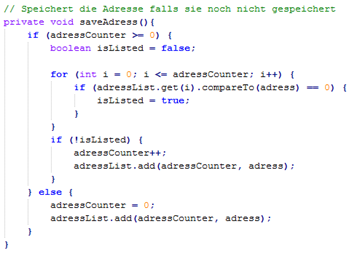
\includegraphics[width=0.8\textwidth]{3Vorgehen/imag/app_saveAdress.png}
    \caption{Sourcecode saveAdress}
	\label{app_saveAdress} 
\end{figure}

Der adressCounter wird mit dem Wert -1 initialisiert. Werden die ersten Daten mit der vorgegeben Struktur empfangen wird die Funktion automatisch die Adresse in der adressList an der Stelle 0 speichern. Werden erneut Daten von einem unserer Sensoren empfangen wird zuerst geprüft, ob die Adresse bereits ein Teil der adressList ist. Falls die Adresse noch nicht in der Liste enthalten ist, wird der Index bzw. der adressCounter, erhöht und die Adresse in der Liste gespeichert.\\

Sobald eine Adresse ausgewählt wurde, müssen die zukünftigen Datenpakete überprüft werden, ob sie vom ausgewählten Sensor stammen. Die Funktion checkAdress (siehe Abbildung \ref{app_checkAdress}) überprüft, ob die ausgewählte Adresse der Adresse des Sensors entspricht, welche die neuen Daten gesendet hat. Sollte keine Adresse ausgewählt sein, so wird dies behandelt, als ob der Sensor die richtige Adresse hat.

\begin{figure}[ht]
    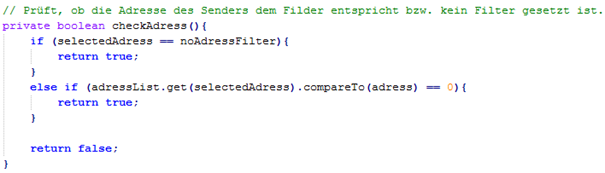
\includegraphics[width=0.8\textwidth]{3Vorgehen/imag/app_checkAdress.png}
    \caption{Sourcecode checkAdress}
	\label{app_checkAdress} 
\end{figure}

Die Benutzerin bzw. der Benutzer muss noch die Möglichkeit haben eine Adresse auszuwählen, dafür wird eine neue Benutzeroberläche (Activity) erstellt. Die neue Activity ist eine List-Activity. Das bedeutet, dass es wird eine Liste von möglichen Adressen angezeigt wird, welche mit einem Klick auf die gewünschte Adresse ausgewählt wird. Anschliessend wird die ausgewählte Adresse an die Haupt-Activity zurückgegeben. In Abbildung \ref{BLEadressauswahl} ist die List-Activity zu sehen, welche eine Adresse zur Auswahl hat. Damit die ausgewählte Adresse von der Haupt-Activity überhaupt empfangen werden kann, musste die List-Activity mit den auszuwählenden Adressen mit folgendem Befehl gestartet werden: startActivityForResult. Die gestartete Activity kann somit ein Resultat, also die ausgewählte Adresse, zurückgeben und die Haupt-Activity kann diese in der Funktion onActivityResult empfangen und abspeichern. Die genaue Ausführung der Übergabe der Adressen sowie die Rückgabe der ausgewählten Adresse kann dem Quellcode entnommen werden.

\begin{figure}[ht]
    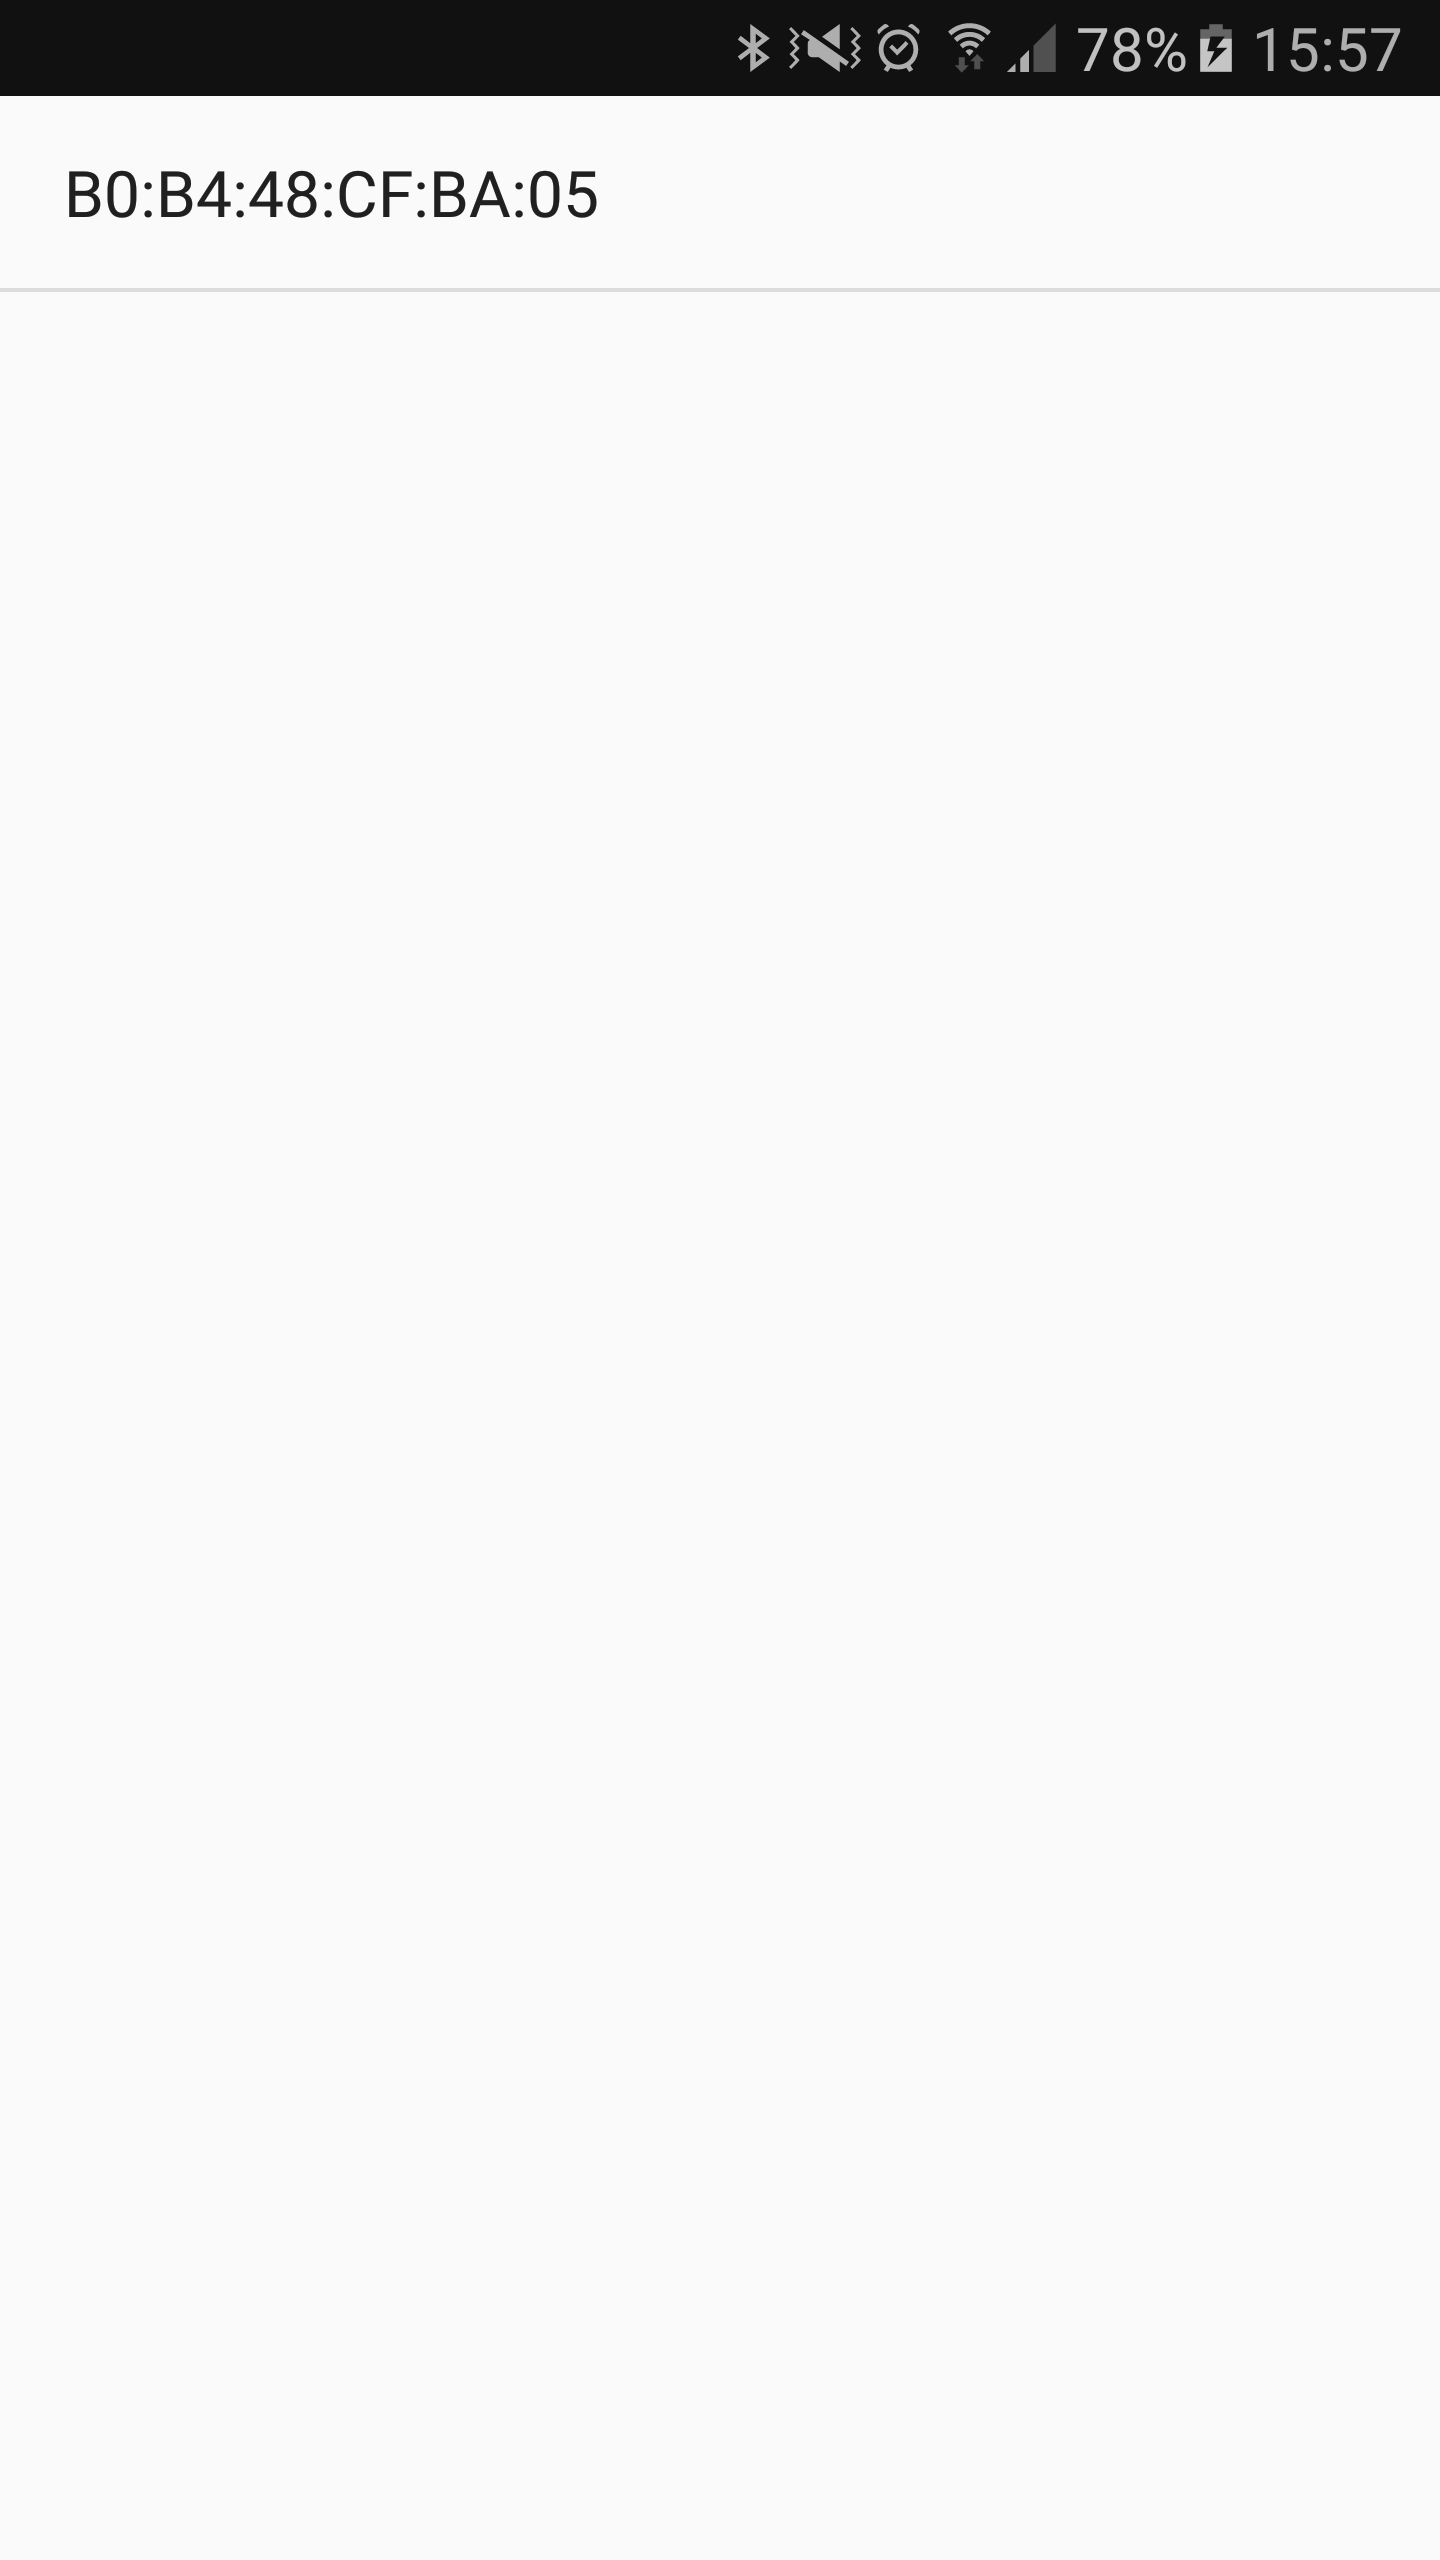
\includegraphics[width=0.2\textwidth]{3Vorgehen/imag/BLEAdresseAuswaehlen.png}
    \caption{Adressauswahl mit nur einer Adresse}
	\label{BLEadressauswahl} 
\end{figure}


\subsubsection{Einheiten}


Die Einheiten der empfangenen Daten sollten ebenfalls einstellbar gestaltet werden. Für diesen Zweck wurden mehrere Enumerationen definiert. Die Enumeration für die Temperatur wird in der Abbildung \ref{app_tempSetting} dargestellt.\\

\begin{figure}[ht]
    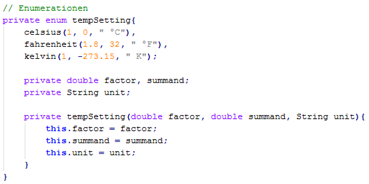
\includegraphics[width=0.8\textwidth]{3Vorgehen/imag/app_tempSetting.png}
    \caption{Sourcecode Enumeration}
	\label{app_tempSetting}
\end{figure}


Es wurden der Enumeration drei Elemente hinzugefügt, welche einen Faktor, einen Offset und einen String mit der geschriebenen Einheit enthalten. Anhand dieser Enumeration kann der Faktor und der Offset einfach zugänglich gemacht werden (\cite{calcTemp})(\cite{calcPressure})(\cite{calcVelocity}). \\

Eine neue Activity wurde codiert, welche drei Spinner zur Auswahl der Einheiten, ein Eingabefeld (EditText) für die Eingabe des Radumfangs und ein EditText für die Kalibrierung der Temperatur zur Verfügung stellt. Die eingestellten Einheiten und die eingetragenen Werte werden über den Speichern-Button an die Haupt-Activity zurückgegeben (siehe Abbildung \ref{onActivityResult}). In der Haupt-Activity werden diese Daten empfangen und abgespeichert und anschliessend zur Darstellung der Werte verwendet. Erst bei der Anzeige der Werte werden die eingestellten Faktoren und Summanden der Enumerationen verwendet.

\begin{figure}[ht]
    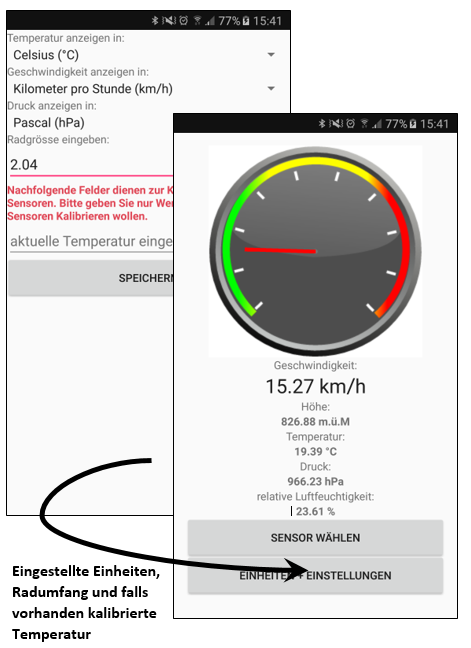
\includegraphics[width=0.2\textwidth]{3Vorgehen/imag/onActivityResult.PNG}
    \caption{Datenübergabe zwischen den Activities}
	\label{onActivityResult} 
\end{figure}

Abschliessend wurde die Activity zur Einstellung der Einheiten noch dahingehend verbessert, dass die eingestellten Einheiten und die eingetragenen Werte bei erneutem Aufrufen der Activity dargestellt werden. Wird die Activity zur Einstellung der Einheiten gestartet, wird ihr die aktuelle Einstellung übergeben und die Spinner und EditText zeigen die zuvor abgespeicherten Werte an. Ein Beispiel: Wenn man in der Activity den Spinner für die Temperatur auf ``Fahrenheit ($^\circ$F)'' einstellt und diese Einstellung abspeichert und dann die Activity dann erneut über einen Druck auf den Button startet, wird beim Spinner für die Temperatur die Einstellung ``Fahrenheit ($^\circ$F)'' angezeigt, da diese Einstellung zuvor abgespeichert wurde.

\begin{figure}[ht]
    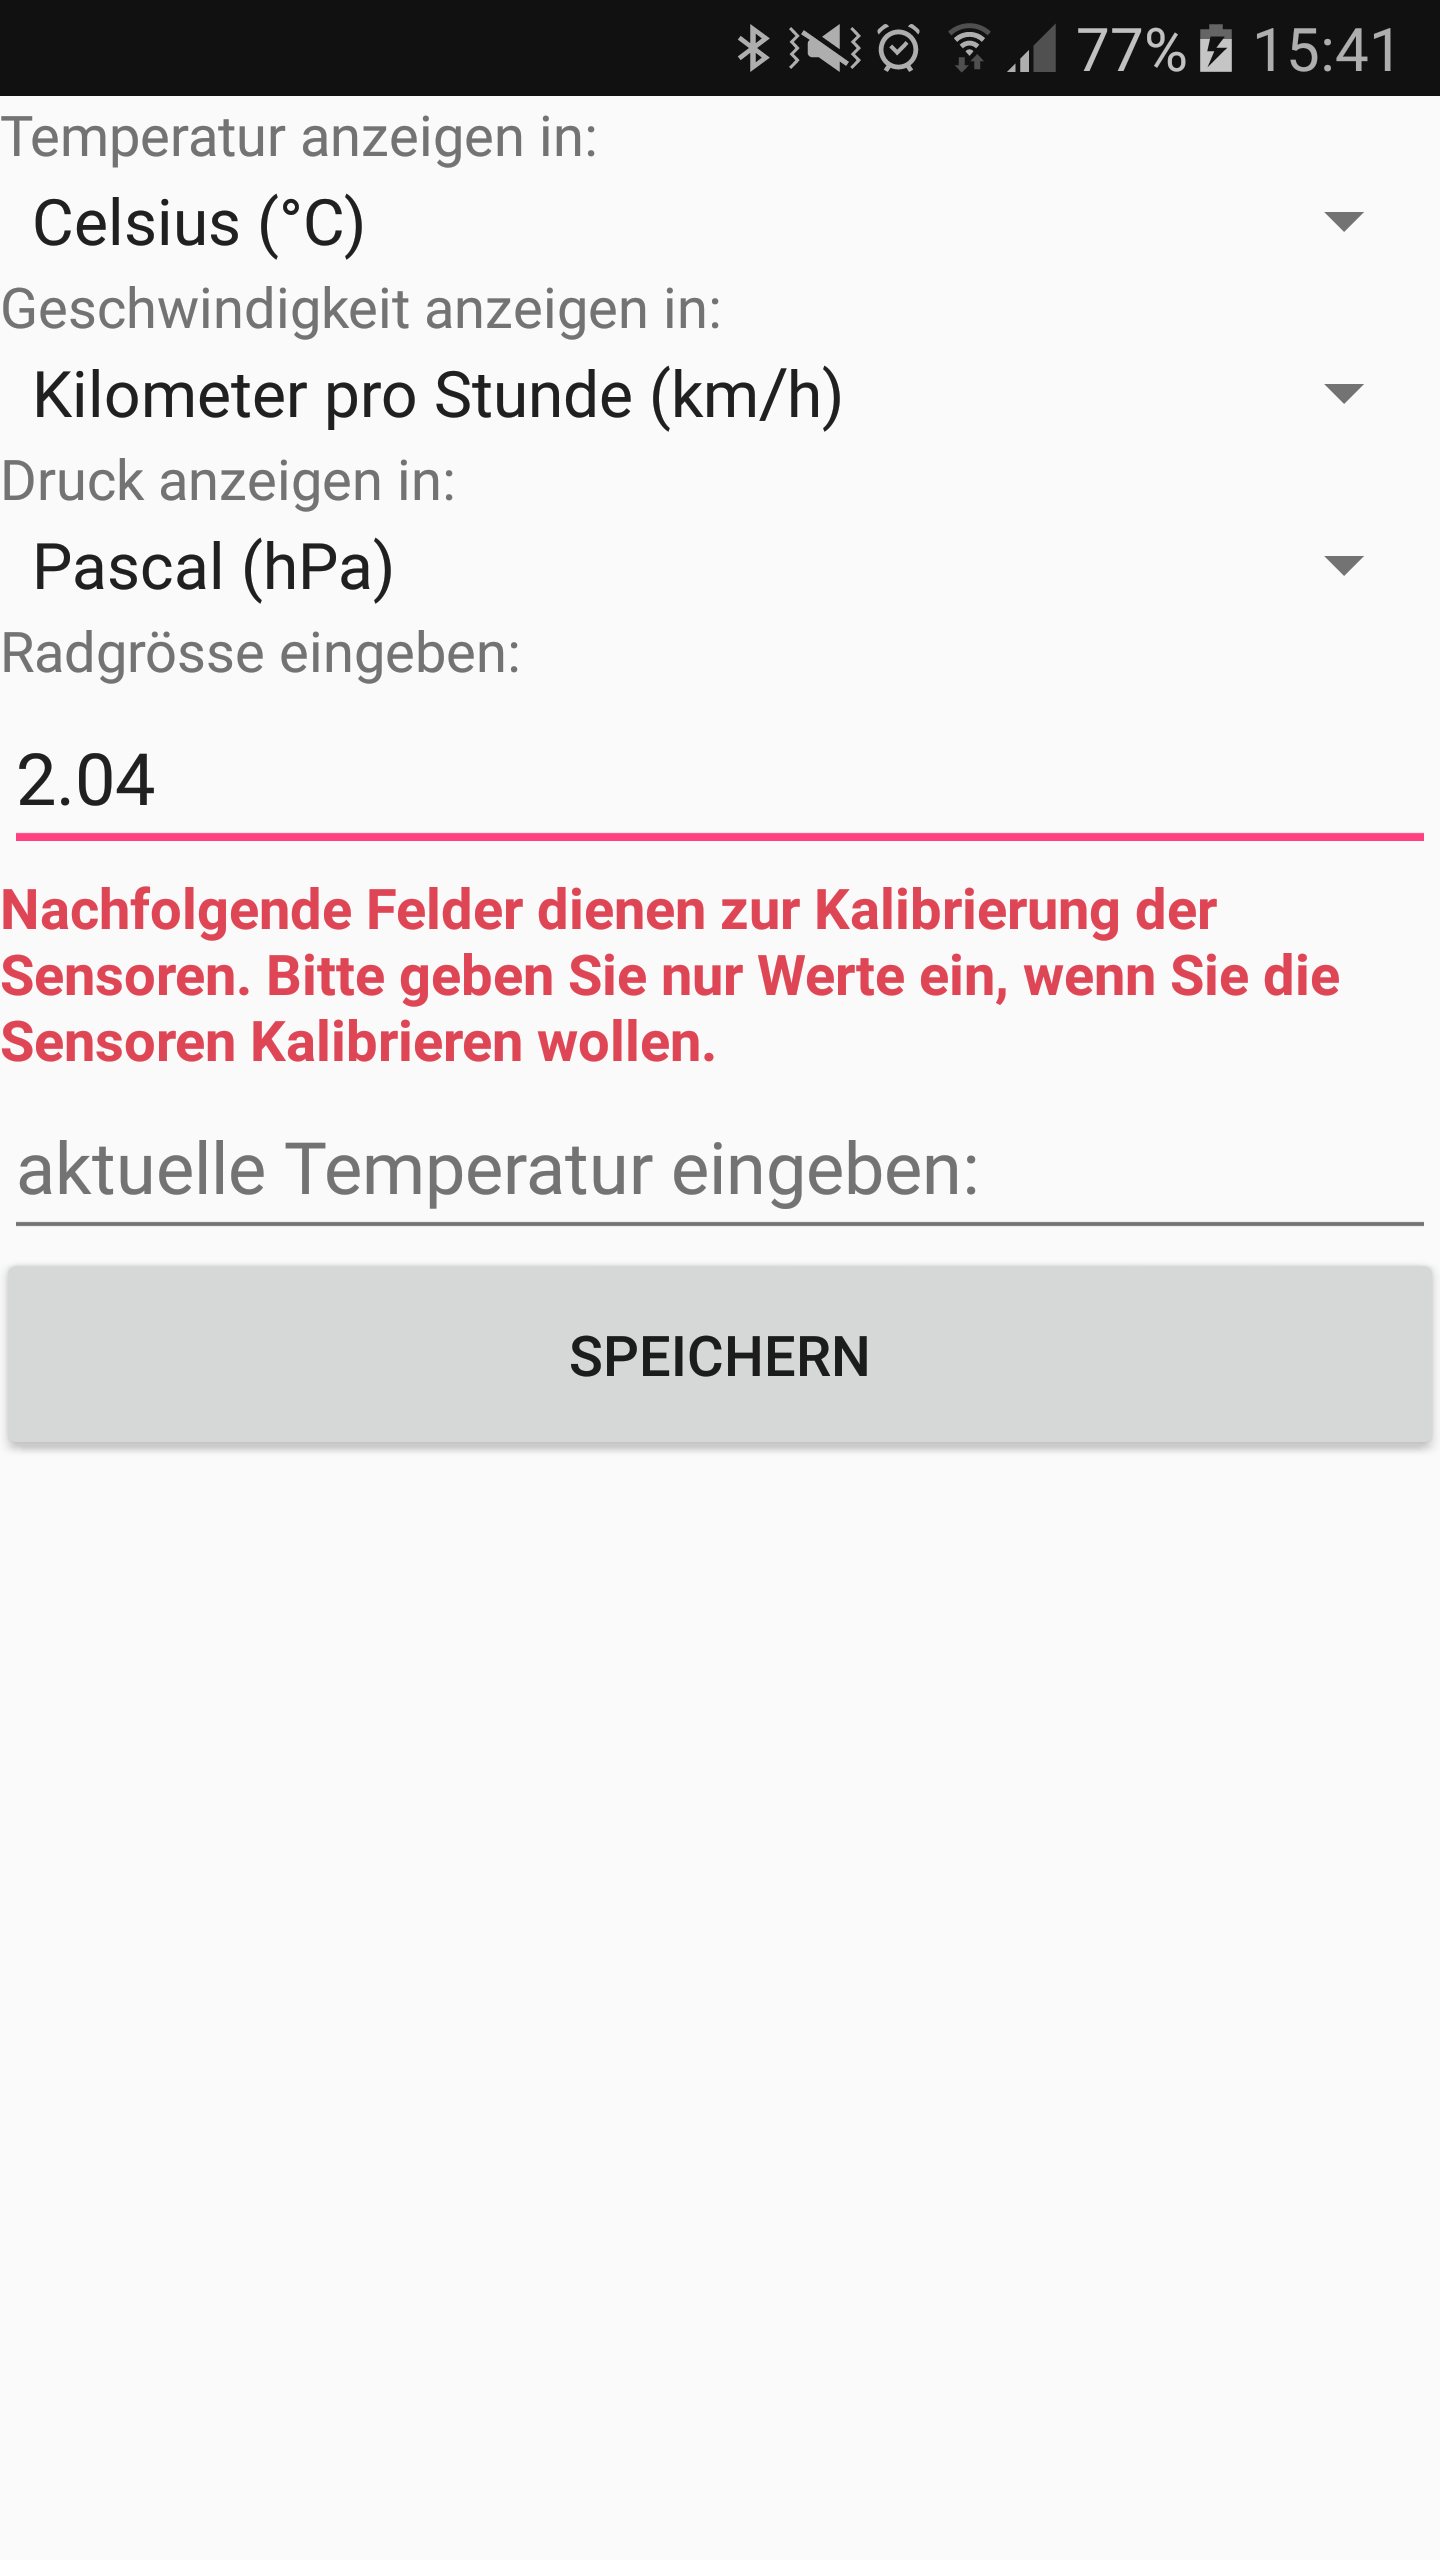
\includegraphics[width=0.2\textwidth]{3Vorgehen/imag/BLEEinheitenUndEinstellungenStart.png}
    \caption{Bildschirm der Einheiteneinstellung}
	\label{BLEEinheitenUndEinstellungenStart} 
\end{figure}


\subsubsection{Kalibrierung}

Während der Entwicklung wurde festgestellt, dass der Wert der Temperatur von der Referenztemperatur abweicht. Aus diesem Grund wurde eine Möglichkeit zur Kalibrierung der Temperatur geschaffen.\\

Die Kalibrierungsmöglichkeit befindet sich in der gleichen Activity, wie die Einstellungen der Einheiten und der Eingabemöglichkeit für den Radumfang. Wird bei dem Textfeld ein Wert eingegeben, so wird diese Temperatur an die Haupt-Activity zurückgegeben. Die Referenztemperatur wird gespeichert und beim Empfang der nächsten Daten wird die automatisch ein Offset berechnet. Dieser Offset fliesst automatisch in die Berechnung der Temperatur ein.

\subsection{Animierter Tachometer}

Es sollte ein Tachometer entwickelt werden, welche eine animierte Tachonadel hat, die die aktuelle Geschwindigkeit anzeigt.

\subsubsection{Funktionsweise}

Bereits in der PA von Manuel König \cite{PA_koenigma} wurde mit der Anzeige von Bilddateien, genauer Bitmaps (.bmp-Datei), experimentiert. Es lag nahe, diese Erfahrung zu nutzen und für dieses Problem eine möglichst einfache Lösung zu generieren. In Android ist es möglich, ein Bitmap in ein Zahlenarray zu laden, dieses Array anzupassen und schlussendlich das Array wieder in ein Bitmap umzuwandeln.

Die Funktion drawTacho liest die Pixel eines Bildes eines Tachometers ohne Tachonadel ein, dreht es und fügt die rote Tachonadel direkt in das Bild ein.

\begin{figure}[ht]
    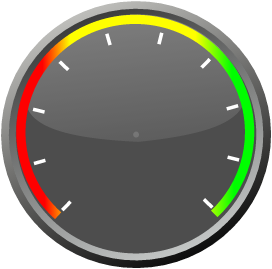
\includegraphics[width=0.2\textwidth]{3Vorgehen/imag/tachometer.png}
    \caption{Tachometer ohne Tachonadel}
	\label{tachometer} 
\end{figure}

Das Bild konnte mit folgender Funktion eingelesen werden:

\begin{figure}[ht]
    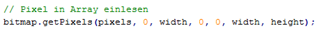
\includegraphics[width=0.2\textwidth]{3Vorgehen/imag/app_getPixel.png}
    \caption{Sourcecode getPixel}
	\label{app_getPixel} 
\end{figure}

Die Bitmap wird in ein eindimensionales Integer-Array eingelesen, die Werte im Array stellen den Farbwert des jeweiligen Pixels dar. Diese Farbwerte können nun verändert werden. Als erstes wurde das ganze Bild gespiegelt, da der rote Bereich des Tachometers auf der rechten Seite angezeigt werden sollte, wie es von anderen Tachometern bekannt ist.

Nach dem Spiegeln des Bildes musste noch die Tachonadel direkt in das Integer-Array eingefügt werden. Die genaue Vorgehensweise wird im nachfolgenden Punkt (\ref{math_tachonadel}) genauer beschrieben.

Aus dem bearbeiteten Integer-Array konnte anschliessend eine Bitmap erstellt werden, welches von der Funktion zurückgegeben wurde. 

\begin{figure}[ht]
    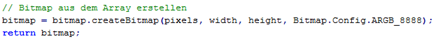
\includegraphics[width=0.8\textwidth]{3Vorgehen/imag/app_createBitmap.png}
    \caption{Sourcecode createBitmap}
	\label{app_createBitmap} 
\end{figure}

\subsubsection{Mathematik der Tachonadel}
\label{math_tachonadel}

\begin{figure}[ht]
    \includegraphics[width=0.8\textwidth]{3Vorgehen/imag/app_drawNeedle.png}
    \caption{Sourcecode Mathematik des Zeigers}
	\label{app_drawNeedle} 
\end{figure}

Die Tachonadel wurde in mehreren Schritten animiert, erst wurde ein Strich mit der Breite von einem Pixel animiert. Die Tachonadel kann als ein Vektor angesehen werden, der im Ursprung des Bitmaps (linke untere Ecke) gedreht und anschliessend verschoben wurde. Die X- bzw. Y-Koordinaten im Bild konnten folgendermassen berechnet werden:

\begin{equation}
	x = \frac{Breite\, des\, Tachometers}{2} + L\ddot{a}nge\, der\, Tachonadel \times \cos(Winkel\, der\, Tachonadel)
\end{equation}

\begin{equation}
	y = \frac{H\ddot{o}he\, des\, Tachometers}{2} + L\ddot{a}nge\, der\, Tachonadel \times \sin(Winkel\, der\, Tachonadel)
\end{equation}

Anschliessend sollte die Tachonadel dicker werden, da ein Strich mit der Breite von nur einem Pixel nicht leicht auf einem hochauflösenden Display zu erkennen ist.

Die Betrachtungsweise, dass die Tachonadel ein Vektor ist, musste angepasst werden. Jeder einzelne Pixel hatte einen Ortsvektor, der angepasst werden musste. Nachfolgende Formel zur Berechnung der Koordinaten nach einer Drehung des Vektors konnte angewendet werden:

\begin{equation}
	x_{neu} = x_{aktuell} \times \cos(\alpha) - y_{aktuell} \times \sin(\alpha)
\end{equation}

\begin{equation}
	y_{neu} = x_{aktuell} \times \sin(\alpha) + y_{aktuell} \times \cos(\alpha)
\end{equation}

Diese Formeln mussten noch mit der Verschiebung in den Mittelpunkt des Tachometers ergänzt werden. Die Koordinaten jedes Pixels der Tachonadel konnten nun berechnet werden und wurden anschliessend mit dem Farbwert für Rot in dem Integer-Array überschrieben.

\begin{equation}
	x_{neu} = \frac{Breites\,des\,Tachometers}{2} + x_{aktuell} \times \cos(\alpha) - y_{aktuell} \times \sin(\alpha)
\end{equation}

\begin{equation}
	y_{neu} = \frac{H\ddot{o}he\,des\,Tachometer}{2} + x_{aktuell} \times \sin(\alpha) + y_{aktuell} \times \cos(\alpha)
\end{equation}

\begin{figure}[ht]
    \includegraphics[width=0.2\textwidth]{3Vorgehen/imag/tachometer_mit_nadel.png}
    \caption{Tachometer mit animierter Nadel}
	\label{tachometer_mit_nadel} 
\end{figure}

\clearpage
\subsection{Modularität der Applikation}

Die Applikationsentwicklung basiert auf einer modularen Struktur.  Dadurch wird eine Weiterentwicklung der Applikation möglich. Ebenfalls wurde beachtet, dass die Applikation sogar in andere Sprachen übersetzt werden kann, dafür wurden alle Texte, die sichtbar sind, in einem File aufgenommen und können zentral abgeändert werden, ohne einen Eingriff in den aktuellen Code. Die verwendeten Texte werden in einem XML-File gespeichtert und mit einer ID versehen, die Applikation greift auf die ID zu. Somit kann der Inhalt des Textes angepasst werden, ohne dass der Sourcecode der Applikation angepasst werden muss.






